
%%
%% To submit your paper:
%[draft,linenumbers]
\documentclass[draft, linenumbers]{agujournal2018}
\usepackage{apacite}
\usepackage{url} %this package should fix any errors with URLs in refs.
\usepackage{textcomp}
\usepackage{amsmath, amssymb, amsthm, wasysym} 
\usepackage{placeins}

\drafttrue
\journalname{Water Resource Research}

\begin{document}

\title{A Global Perspective on Local Meteoric Water Lines: Meta-analytic Insight into Fundamental Controls and Practical Constraints}

\authors{Annie L. Putman\affil{1,2}, Richard P. Fiorella\affil{1}, Gabriel J. Bowen\affil{1, 2}, Zhongyin Cai\affil{3}}


\affiliation{1}{Geology \& Geophysics Department, University of Utah}
\affiliation{2}{Global Change \& Sustainability Center, University of Utah}
\affiliation{3}{Institute of International Rivers and Eco-security, Yunnan University}

\affiliation{1}{383 F.A. Sutton Bldg. 115 S. 1460 E., Salt Lake City, UT 84112-0102, US}
\affiliation{2}{234 F.A. Sutton Bldg. 115 S. 1460 E., Salt Lake City, UT 84112-0102, US}
\affiliation{3}{Yunnan University, Kunming, Yunnan 650091, CN}
\correspondingauthor{Annie Putman}{putmanannie@gmail.com}

\begin{keypoints}
\item LMWLs exhibit sensitivity to record length in most regions
\item LMWLs exhibit spatial variation corresponding to hydroclimatic variability
\item Isotope-enabled climate model LMWLs exhibit biases relative to observational LMWLs 
\end{keypoints}

\begin{abstract}
Local meteoric water lines (LMWLs) represent the site-specific long-term covariation of hydrogen and oxygen stable isotope ratios. LMWLs have practical utility as a hydrologic framework and as benchmarks for evaluating hydroclimatic processes in isotope-enabled climate models. In this manuscript, we characterize the global distribution of LMWLs and compare them to LMWLs from model data. To evaluate the sensitivity of the covariance of stable isotope ratios to dataset length, we paired timeseries rarifaction with Bayesian ellipse estimation. We then applied a threshold of 48 months and estimated LMWLs at 398 sites in 25 K{\"o}ppen climate classes using orthogonal distance regression. Slopes ranged from 4.8 to 10.9, with an average of 7.64 $\pm$0.64. Intercepts ranged from -24\textperthousand to 27\textperthousand, with an average of 6.85 $\pm$6.2\textperthousand. We identified three processes: 1) sub-cloud evaporation of rain, 2) atmospheric re-moistening by rainfall evaporation, and 3) conditions of snow formation as important controls on slopes and intercepts in arid, humid, and seasonally snowy regions, respectively. We compared observational LMWLs with those from a suite of isotope-enabled climate models. At arid and snowy sites, model data produced higher slopes and intercepts than observational data. At humid sites, model data exhibited dampened variability in slopes and intercepts relative to observational data. These results indicate potential for improvement in the precipitation and/or isotope parameterizations of raindrop evaporation, advection of re-evaporated water, evapotranspiration fractionation, and supersaturation in mixed-phase clouds. This meta-analysis demonstrates LMWLs utility for identifying specific hydroclimatic and isotopic processes in observations and models.
\end{abstract}
%%
%% Start line numbering here if you want
%%
%\linenumbers

%% main text
\section{Introduction}
\label{S:1}
The global linear relationship between the stable isotopic ratios of hydrogen ($\delta^{2}H$) and oxygen ($\delta^{18}O$) in meteoric waters was first documented by~\citet{Craig1961}, and yielded the global meteoric water line (GMWL), defined as $\delta^{2}H = 8*\delta^{18}O + 10$. Later, \citet{Rozanski1993} delved into the variability in local meteoric water lines (LMWL) by comparing the $\delta^{2}H$-$\delta^{18}O$ relationships of monthly scale samples at selected Global Network of Isotopes in Precipitation (GNIP) sites. This analysis sorted the slopes into one group comprised of continental and coastal stations, and one comprised of marine stations. Slopes between about 5.5 and 8 were reported, with a single exception at a maritime site having a slope of 2.8 due to low variance in the data. Findings by both~\citet{Craig1961} and \citet{Rozanski1993} suggested that 1) the linear statistical relationship of hydrogen to oxygen isotopic ratios varies spatially, and 2) variation in the slope may hold information about seasonal climatology of the site.

Local meteoric water lines are a simplified, intuitive representation of the average $\delta^{2}H$-$\delta^{18}O$ relationship at a site. Coupled with information about the range of isotope ratios, a LMWL can provide a reference framework for interpreting the isotope ratios measured in terrestrial (e.g., ground, river, or lake) and biologically derived (e.g., stem, leaf) waters. Specific applications include estimating the seasonality of groundwater recharge \citep{Jasechko2014} and the evapoconcentration (isotopic alteration due to preferential evaporation of light isotopologues) of lake waters \citep{Bowen2018}, as well as the seasonality of soil water supplied to plants \citep{Brooks2010} or used in carbonate formation \citep{Huth2019}. Local meteoric water lines can also provide useful, process-oriented checks on hydrology and isotope routines in isotope-enabled atmospheric circulation models (iGCMs).  Despite all of the applications of LMWLs discussed above, less effort has been put towards understanding the global variability and controls on LMWLs. For example, LMWLs may be assumed to be regionally representative and insensitive to record length or collection time period, so a precipitation dataset from a neighboring state or country, collected decades prior may be used to estimate the LMWL for a study. This scenario may be valid for some projects but not others. This global meta-analysis can provide researchers with information for evaluating whether their LMWL parameters are consistent with the LMWL parameter range expected for a region or hydroclimate, and the length of spatial autocorrelation for LMWL parameters in a region.

LMWLs are based on datasets that represent the long-term distribution of $\delta^{2}H$ and $\delta^{18}O$ at a site. Thus, the first aim of this manuscript is to provide an estimate the minimum number of years of sampling required to establish a LMWL that is representative of the multidecadal distribution of $\delta^{2}H$ and $\delta^{18}O$. The second aim of this manuscript is to report the spatial structure and provide bounds on the global distribution of LMWL slopes and intercepts using a compiled, global dataset. We interpret the observed spatial structure in terms of specific hydroclimatic processes characteristic of climate types. The third aim of this manuscript is to evaluate the representation of those processes in iGCMs by comparison of LMWLs from a suite of models to the global observational LMWL dataset. 

\subsection{Meteoric Water Line fundamentals}
The $\delta^{2}H$-$\delta^{18}O$ covariance summarized by LMWL results from the interplay of water isotope systematics and hydroclimatic seasonality at a site.  The variability in the $\delta^{2}H$-$\delta^{18}O$ pairs results from water isotope fractionation during phase changes (e.g., evaporation, condensation, and deposition) and across humidity gradients (e.g., vapor diffusion from a saturated water surface into dry air above \citep{CraigGordon1965}). Fractionation factors, which quantify the strength of the isotopic sorting between phases, are controlled by both temperature and humidity, where the isotopic sorting effect is greater at cooler temperatures and lower humidities~\citep{Majoube1971, Cappa2003}. The majority of the meridional and altitudinal variation in observed isotopic values arises from variation in Rayleigh distillation: the progressive rainout of heavy isotopologues driven by equilibrium fractionation during the evolution of a precipitating airmass \citep{Gat1996}. 

LMWLs are often evaluated in the context of their deviation from the GMWL, which is used as the `expected' equilibrium relationship, where the slope is assumed to arise from the ratio of equilibrium fractionation factors. However, the GMWL is defined primarily by spatial variability, and its slope of 8 reflects the average global spatial relationship between $\delta^{2}H$ and $\delta^{18}O$ in precipitation. This distinction is important because of the variation in the expected equilibrium fractionation ratio of $\delta^{2}H$ to $\delta^{18}O$ at different temperatures, as well as a mathematical non-linearity in $\delta$ notation \citep{Dutsch2017}. As a result, LMWLs with slopes different than 8 may simply indicate predominantly equilibrium processes in a particular temperature and/or isotope composition range. 

Alternatively, LMWL slopes different than 8 may indicate that at least one season is characterized by precipitation affected by non-equilibrium processes. In this framework, non-equilibrium processes are identified with the deuterium-excess parameter, defined as $d = \delta^{2}H - 8* \delta^{18}O$, where $d$ for the $\delta^{2}H$ and $\delta^{18}O$ pairs falling on the GMWL is 10~\citep{Dansgaard1964}. We can apply our understanding of $d$ systematics in different hydroclimates and seasons to interpret LMWL variability. 

The first example of a non-equilibrium process is diffusion across a humidity gradient. This occurs when rain droplets partially evaporate into dry air~\citep{Stewart1975, LeeFung2008}, leading to isotopically heavier precipitation at the ground than at the cloud base and lower $d$. As a secondary effect of this process, the re-evaporated water vapor has high $d$. If this re-evaporated vapor supplies subsequent precipitation, a process called `re-moistening'~\citep{Noone2012} which is common in tropical regions~\citep{Worden2007}, the downstream precipitation may be characterized by high $d$. This has been observed in $d$ gradients across the Amazon Basin~\citep{Martinelli1996} and in a site-specific study of Costa Rican precipitation~\citep{SanchezMurillo2017}. High $d$ in water vapor over continents may also arise from the evaporation of land surface sources, like lakes and soil waters \citep<e.g.,>{Feng2016} and is evidenced by the evapoconcentration of lakes~\citep{Bowen2018}.

The second example of a non-equilibrium process is the formation of precipitation in mixed-phase clouds, where vapor is supersaturated over ice~\citep{JouzelMerlivat1984}, and ice grows by deposition at the expense of evaporating supercooled liquid droplets. In this case, the vapor supplied for deposition will have higher $d$, which is partially transferred to the ice, leading to high $d$ in precipitation from mixed phase clouds. Though mixed phase clouds occur in all seasons and latitudes, the high $d$ from the non-equilibrium process is observed primarily in snow formed from mixed phase clouds. 

For precipitation characterized by the processes described above, the $d$ measured in precipitation will reflect the processes during precipitation formation, as well as the upstream processes that control the $d$ of the vapor supplying precipitation. For example,~\citep{Ciais1994} model the evolution of $d$ during the progressive rainout of an airmass moving inland in Antarctica and find that $d$ increases along the trajectory. Likewise, precipitation in a dry region with vapor supplied by continental recycling characterized by high $d$ may exhibit higher $d$ than a dry region supplied primarily by advection of marine boundary layer vapor. Upstream effects on the $d$ of vapor introduce variability into the $d$ that must be considered when interpreting measured $d$ in terms of hydroclimatic processes.
\section{Methods}
\subsection{Water isotope data processing}
\label{sec:processing}
Our analysis leveraged a global monthly-scale $\delta^{2}H$ and $\delta^{18}O$ dataset obtained from the~\citet{spatialwi} including data from the Global Network of Isotopes in Precipitation~\citep{GNIP} and others. The $\delta$ values refer to the Vienna Standard Mean Ocean Water (VSMOW)-normalized heavy-to-light isotope ratios~\citep{Coplen1996} ($\delta = \frac{R_{SA}-R_{VSMOW}}{R_{VSMOW}}$, where $R = \frac{^{18}O}{^{16}O}$ or $\frac{^{2}H}{^{1}H}$), and are reported in~\textperthousand.

Data from projects sampled at sub-monthly temporal resolution were averaged to monthly scale using event-scale precipitation amount data. Whenever possible, the precipitation amount data came from the same study as the water isotope data collection. However, in cases where the event-scale water isotope data were presented without precipitation amount information,  we used gridded daily precipitation data from the CPC Global Unified Precipitation dataset~\citep{CPCprec}. The resulting monthly-scale processed dataset (available in the supplemental information) was used either in full or subset for all following analyses.

\subsection{Characterizing the long term isotope distribution at a site}
A LMWL that is characteristic of a site reflects the long term distribution of $\delta^{18}O$ and $\delta^{2}H$ at the site. However, due to lack of data availability, it is common practice to estimate LMWLs with just a few years of data~\citep{Benjamin2005} or with a combination of precipitation and precipitation-archiving waters~\citep{Kopec2018}. Our analysis establishes guidelines on the amount of time required to adequately characterize the long term isotope distribution at a site. To do this, we employed Bayesian ellipse estimation, a robust method for representing the covariance structure of bivariate systems~\citep{Jackson2011}, which has been demonstrated to be unaffected by small sample sizes. The method is described below, and also included in a flow chart available in the supplemental information.

To estimate the sensitivity of the covariance of $\delta^{18}O$ and $\delta^{2}H$ at a site to record length, we calculated ellipses from rarified subsets of data at sites with more than 10 years (120 months) of water isotope samples. This dataset consisted of 162 sites from 8 projects at 20 K{\"o}ppen climate classifications, with 95\% of sites from the Global Network of Isotopes in Precipitation~\citep{GNIP}. 

The training datasets for the Bayesian ellipse estimations were 18, 24, 30, 36, 48, 60, 72, 84, 96, 108 and 120 months long. The training datasets are termed `subtimeseries' because the initial date is randomly chosen, and all the subsequent months up to the training dataset length are included. This method for subsampling the full dataset aims to preserve characteristics of timeseries, including seasonality and data gaps that might be lost with totally random subsampling. Our analysis allowed for sampling gaps of any time length, reflecting the practical limitations associated with record discontinuity at many long term monitoring sites. However, to ensure that the subtimeseries adequately represented seasonality at the site, we required that the subtimeseries include at least 3 samples in each 3-month meteorological season where at least 10 mm of precipitation is expected. These samples did not have to occur consecutively. To account for the reasonable range of ellipse parameter estimates, 10 unique training datasets were generated for each subtimeseries length tested. An exception occurred for some 120 month subtimeseries: at sites with 129 months or fewer we could not generate 10 unique subtimeseries, thus, only the unique subtimeseries were analyzed. An ellipse based on the complete dataset was calculated at each site for comparison.

The Bayesian inference ellipses were estimated using the `pymc' module, following the methods described in~\citet{Jackson2011} and recreates the open access SIBER R package. The method will be described briefly, and is also presented as a flow chart (Figure S1). Generally, this method derives numerous (2500) estimates of $\delta^{18}O$ and $\delta^{2}H$ means and the $\delta^{18}O$-$\delta^{2}H$ covariance matrix from a training dataset, a specified, vague prior probability, and a likelihood function. In this analysis, the $\delta^{18}O$ and $\delta^{2}H$ means were assigned vague normal priors, and the covariance matrix was specified with a vague inverse Wishart prior. Sampling was performed for 6000 iterations, with 1000 iterations used as a burn in period, and resulting samples were thinned by 2.  Two chains were run for each model sampling instance, and the chains were compared using Gelmen-Rubin metrics for estimated variance deflation (pymc.gelmen\_rubin()) and an unequal variance t-test of the sample means (scipy.stats.ttest\_ind(equal\_var = False)). If the two chains were sufficiently similar, the sampling results were accepted. We then combined the chains and took the means of the $\delta^{18}O$ and $\delta^{2}H$ estimate distributions to estimate the ellipse centerpoint. The instances of covariance matrices were converted to ellipse major and minor axis lengths and angles of rotation using eigen decomposition, and we calculated the average of the distribution of these quantities. The estimation of the ellipse and subsequent comparison metrics account for uncertainty in the sampled data and naturally incorporate error arising from the sampling process, which are not present in a frequentist estimate of the mean and covariance structure of a dataset. We compare ellipses as opposed to the means and covariance matrices because they allow us to use metrics of overlap and total area, providing a simple, descriptive summary statistic for the similarity or difference of the distribution of two datasets.

The rarified timeseries were evaluated in terms of the standardized ellipse overlap area (Equation~\ref{eq:Eover}), defined as the area of intersection between ellipse estimated from the data subtimeseries ($A_{Esub}$) and ellipse estimated from full timeseries ($E_{Eall}$), normalized to the union area of the two ellipses. This is because the subtimeseries ellipse is often larger than the ellipse calcualted from the full timeseries due to increased uncertainty at smaller sample sizes.
\begin{equation}
A_{Eover} = \frac{A_{Eall}\cap A_{Esub}}{A_{Eall} \cup A_{Esub}}
\label{eq:Eover}
\end{equation}
Ellipse areas, intersection, and overlap were calculated using tools provided by Python's `shapely' module. Greater overlap relative to total area covered indicates similar means and covariance structure among two different datasets.

\subsection{LMWL calculation}
The Bayesian ellipse estimation method was used to evaluate the sensitivity of $\delta^{18}O$-$\delta^{2}H$ covariance to record length. Based on the distribution of $A_{Eover}$ values at each subtimeseries length and dataset coverage (Figure~\ref{fig:ellipse}), we established a threshold for minimum record length for this project of 48 months and extracted a subset of the processed data. From that subset, we calculated LMWLs  for these sites using an orthogonal distance regression approach (`ODR()' in the python `scipy.odr' module). This approach does not assume dependency of $\delta^{2}H$ (y variable) on the $\delta^{18}O$ (x variable), and allows for error in both $\delta^{2}H$ and $\delta^{18}O$~\citep{Crawford2014}. The error corresponding to the $\delta^{2}H$ was assumed to be $\pm$ 0.5\textperthousand\, and for $\delta^{18}O$ was assumed to be $\pm$ 0.1\textperthousand\, corresponding to analytical error estimates. This analysis did not weight by the monthly precipitation fluxes when estimating the LMWLs. Including precipitation fluxes is useful when linking precipitation seasonality to ground and soil water resources~\citep{Hughes2012, Wang2018} but is less appropriate in characterizing atmospheric processes and hydroclimatic controls on water isotope seasonality. 

\subsection{Isotope-enabled GCM LMWL calculation}
The final component of this study is to compare observed LMWL parameters to those simulated by iGCMs to evaluate how well the models simulate the processes controlling both the hydroclimate and the water isotope fractionation. We used results from an ensemble of eight iGCM simulations, with native resolution and model and isotope references documented in Table~\ref{tab:modrefs}. Briefly, these included the Stable Water Isotope iNtercomparison Group 2 ensemble~\citep{Risi2012}, and two more recent simulations using CAM5~\citep{Nusbaumer2017} and ECHAM5~\citep{Steiger2017}. All eight simulations were forced with historical sea surface temperatures and have a common overlap period of 1980-2001. Precipitation isotopologue fluxes were regridded from their native resolution (Table~\ref{tab:modrefs}) to a common 1\textdegree x1\textdegree\ grid using a second-order globally mass-conservative interpolation scheme~\citep{Jones1999} before conversion to standard delta notation. At each grid point that corresponds to an observational data sampling site, we estimated LMWL slope and intercept values using orthogonal distance regression on monthly data across the common 21-year period. Though we do not expect a model grid cell to match a point measurement site, in most locations the hydroclimatic patterns observed at the site scale are also expected to be reflected at the broader spatial scales represented by the grid cell. The exception to this generalization is in cases of sharp climate gradients which cannot be represented in the model at the native 2-3\textdegree\ resolutions, such as close to major mountain ranges.  

\section{Results and Discussion}
\subsection{Impacts of timeseries length on variability in LMWL estimation}
Bayesian ellipse estimation resulted in up to 1620 ellipse calculations at each subtimeseries length (18-120 months) and a maximum of 12,960 total possible ellipse calculations across all eligible sites, including the ellipse estimations from full timeseries. Similarity between the subtimeseries and full timeseries ellipses increased with longer subtimeseries lengths (Figure~\ref{fig:ellipse}), where the median values for each subtimeseries followed an exponential curve fit ($y =0.38+ 0.508 (1-e^{x/120}$). Although we do not expect exact matches between any subtimeseries length and the full timeseries since there is a random component of variability arising from the Bayesian method of estimation, the additional variability suggests the importance of interannual and decadal variability in the timeseries affects the covariance structure of $\delta^{18}O$ and $\delta^{2}H$. This isotopic variability may be driven by hydroclimatic changes, or in response to cyclicity of teleconnections~\citep{Baldini2008, Liu2011}. 

The sensitivity of the covariance of $\delta^{18}O$ and $\delta^{2}H$ to record length suggests that for analyses that require a water isotope distribution closely resembling the long term distribution, such as characterization of recharge of deep groundwater aquifers or for paleoclimate applications, longer records improve the representativeness of the LMWL. However, for questions where the terrestrial water archive has a shorter residence time, like characterizing the source waters for plant or animal tissue, studies may benefit from using a meteoric water line from a dataset collected during the period of study. Nonetheless, we observe that interannual-to-decadal scale variations in the $\delta^{2}H$ and $\delta^{18}O$ distributions can be large and should be expected to influence metrics like LMWL. Thus, we recommend that researchers incorporate considerations of timescale and coeval collection when designing projects that utilize a LMWL framework.  

We applied a threshold of 48 months of data to characterize the long-term bivariate distributions of $\delta^{18}O$ and $\delta^{2}H$ at a site. We allowed sampling gaps of any length. Among long time series (\textgreater 240 month), slopes and intercepts for 48-month subtimeseries were evaluated to gauge the temporal variability in LMWL parameters. This dataset is available in the supplemental information. Among these sites, the difference between the highest and lowest slopes exhibited a median of 1.2, with differences as low as 0.36 and as high as 4.4. The difference between the highest and lowest intercepts exhibited a median of 10.05\textperthousand, a minimum of 4.0\textperthousand\ and a maximum of 30.9\textperthousand. The highest temporal variability in LMWL parameters tended to occur at sites that experienced wet-dry seasonality or were mid-ocean island sites characterized by high variability among seasons and years. Sites characterized by warm-cold seasonality tended to exhibit less variability across the timeseries. 

The results summarized in Figure~\ref{fig:ellipse} suggest that our choice of lower data threshold will introduce some noise into our analysis of the spatial distribution of LMWL slopes and intercepts. However, as shown on the secondary axis, the relatively flexible criterion of 4 years allows us to retain spatial coverage at a reasonable number of sites relative to a more restrictive record length criterion. Retaining global coverage at a broad range of hydroclimates is a concern for this dataset, as many of the longest global precipitation isotope records come from European sites, and records tend to be short in sparsely sampled regions like central Africa or Siberia. This analysis leverages a large global dataset, where 40\% of our sites have more than 10 years of data, to investigate zonal and climate region patterns. Thus, noisiness that may arise from shorter datasets is mitigated by pooling data by climate class. 

\subsection{Local Meteoric Water Line values and hydroclimatic mechanisms}
\label{sec:LMWLhydroclim}
Using the 4-year criterion, we created a data subset (full dataset described in Section~\ref{sec:processing}) including 55,923 site-months of water isotope data at 398 sites. The Global Network of Isotopes in Precipitation~\citep{GNIP} supplied 87\% of the site-months, with an additional 107 sites from 22 other projects~\citep{Kurita2004, Harvey2005, KuritaJAMSTEC, Price2008, Harris2010, Peng2010, Abiye2013, Hughes2013,  Moerman2013,  Scholl2014, Yamanaka2015, MayerPC, Braun2017, BrooksJRPC01, CsankPC01, Putman2017, Chen2018, FengPC01, EhleringerPC01, GrimesPC, WassenaarPC}. 

Among this subset of sites, LMWL slopes ranged from 4.8 to 10.9, with an average and standard deviation of 7.64 $\pm$ 0.64. Intercepts ranged from -24 \textperthousand\ to 27 \textperthousand, with an average and standard deviation of 6.85 $\pm$ 6.2 \textperthousand. Both slopes and intercepts had the lowest standard error at sites with large variances in $\delta^{18}O$ and $\delta^{2}H$. This means that sites that experience wide ranges of isotope ratios tend to have a more well defined LMWLs than sites with less variance in observed isotope ratios. This dataset containing site metadata and LMWL parameters is available in the supplemental information. 

Meteoric water line slope and intercept values both showed coherent spatial structure (Figure~\ref{fig:lmwlpoints}), which appears to be associated with regions of contrasting hydroclimate (Figure~\ref{fig:zonalboxplot}). Humid tropical (K{\"o}ppen class A) and temperate regions (K{\"o}ppen classes Cf, Cw) were characterized by slopes between 8 and 9, and intercepts of 5 to 20\textperthousand.  Subtropical arid or seasonally hot and dry regions (K{\"o}ppen class B and Cs) were characterized by slopes between 5 and 7, and intercepts between 0 and 15\textperthousand. Humid temperate (K{\"o}ppen class Cf), seasonally snow-dominated regions (K{\"o}ppen class D), and cryosphere (K{\"o}ppen class E) sites tended to have slopes between 7 and 8, and the lowest intercepts, between -20 and 5\textperthousand. 

LMWLs at low latitude warm or hot sites (K{\"o}ppen climate classes A, B and Cs) tend to be anchored by minimum $\delta^{18}O$ and $\delta^{2}H$ values lying on or close to the GMWL, with $d$ close to 10 (Figure~\ref{fig:seasonaldex}, panel (b)), but the heaviest $\delta^{18}O$ and $\delta^{2}H$ at the site often lie well above or below the GMWL (Figure~\ref{fig:seasonaldex}, panel (a)), giving slopes greater or less than 8, respectively. Sites with high slopes tend to cluster in tropical regions (K{\"o}ppen class A), and those with low slopes in arid and seasonally hot and dry zones (K{\"o}ppen classes B and Cs). High slopes could be supported by re-moistening of the atmosphere by evaporation of rainfall or canopy intercepted water~\citep{Noone2012} by upstream precipitation. This mechanism is in keeping with the estimates of~\citet{Worden2007}, who found that as much as 20\% to 50\% of rainfall near convective clouds evaporates. This mechanism has a cumulative effect, with increasing $d$ towards basin interiors reflecting increased proportions of re-evaporated vapor with increased distance from the coast~\citep<e.g.,>{Martinelli1996}. Plant transpiration, sub-cloud evaporation, and mixed phase cloud processes occurring in tall convective towers within tropical basins are all mechanisms that can counterbalance the high $d$, leading to slopes closer to 8. The observed low slopes in arid regions could be supported by sub-cloud evaporation into dry air, a process which is enhanced for smaller droplet size~\citep{LeeFung2008}, with the limit that at very small droplet sizes, droplets will not reach the ground. This mechanism may be affected by upstream processes including mixing or Rayleigh-distillation based airmass evolution that can work constructively or destructively to yield low $d$. For example, precipitation from high $d$ vapor, from continental recycling or rapid evaporation from the ocean that experiences sub-cloud evaporation may not exhibit very low $d$, whereas low $d$ vapor, such as vapor from a humid, cool oceanic boundary layer may exhibit less sub-cloud evaporation but produce the same $d$. However, the range of seasonal average $d$ observed in our dataset matches the range of $d$ from three studies~\citep{Chen2015, Wang2016, Graf2019} that measured precipitation isotope ratios and modeled a strong contribution of sub-cloud evaporation to the observed $d$.

Seasonally snowy and polar regions (K{\"o}ppen class D) tend to be characterized by very large seasonal variability (range \textgreater\ 25\textperthousand\ in $\delta^{18}O$), resulting from the warm season reliance on regional continental vapor, and the cold season dependence on distal oceanic vapor sources~\citep{Putman2017, Bailey2018} and thus potential for Rayleigh distillation. At most continental sites cold season $d$ is higher than warm season $d$. Wintertime $d$ tends to be lower on the western side of the continent and higher on the eastern side of a continent (in our dataset all D class sites are in the Northern hemisphere), possibly reflecting the effects of Rayleigh distillation on $d$ by altering the humidity of the precipitating clouds or the $d$ of the airmasses producing precipitation~\citep{Ciais1994}. The higher wintertime $d$ arises from precipitation formed in mixed-phase clouds, where ice grows by deposition at the expense of supercooled liquid droplets~\citep{JouzelMerlivat1984}, and minimal alteration of snow and ice below cloud base. In select locations that experience lake effect snow, such as the Great Lakes region of North America and certain sites in Japan, wintertime $d$ is even higher (Figure~\ref{fig:seasonaldex}, panel (d)), resulting from rapid evaporation of lake or ocean water into dry, cold continental air~\citep<e.g.,>{Corcoran2019}.Lake effect snow contributes to lower slopes at these select sites. Warm season $d$ varies widely for continental sites, and some sites exhibit low $d$. This suggests moderate to substantial influences of sub-cloud evaporation during the warm season at specific sites (Figure~\ref{fig:seasonaldex}, panel (c)). Thus, among continental, seasonally-snowy sites, low slopes may be driven by the high $d$ of wintertime precipitation associated with lake effect snow, or may be driven by low $d$ of summertime sub-cloud evaporation combined with higher $d$ associated with wintertime snow. 

Our analysis indicates that spatial variation in slopes and intercepts arises from variation in hydroclimatic and isotopic mechanisms. From this analysis, we propose a conceptual model for idealized LMWL scenarios from different hydroclimatic regions, including tropical, arid, and seasonally snowy (Figure~\ref{fig:LMWLschematic}).  We compare these idealized LMWL scenarios with the GMWL and contextualize the LMWLs with the $\delta^{18}O$-$\delta^{2}H$ biplot region inhabited by all LMWLs. In general, the mechanisms most important for defining a LMWL occur during the seasons responsible for $\delta^{18}O$-$\delta^{2}H$ extrema. These may correspond to warm and cold seasons in the mid and high latitudes, and wet and dry seasons in the tropics and sub-tropics. In this section, we have explored the mechanisms responsible for the most extreme observed LMWL slopes and intercepts, including sub-cloud evaporation, continental recycling and mixed-phase cloud processes which may raise or lower the slope, depending on the season. These processes may also be at play in other climatic regions that are not discussed explicitly above. For example, polar sites (K{\"o}ppen class E), depending on their hydroclimate, may have a season of high $d$ due to mixed phase cloud processes. As well, temperate dry winter sites (K{\"o}ppen class Cw) may experience either sub-cloud evaporation or continental recycling, depending on the humidity and temperature of the warm season. Spatial variation in the upstream processes (e.g., proximity to ocean, upstream Rayleigh distillation, continental resupply) may account for some of the observed spatial variability. Variations in the strength of the processes discussed in this section may also be responsible for the temporal variability in LMWL observed in long datasets. For example, mixed phase cloud processes occurring during the warm season of polar regions (K{\"o}ppen class E) like Antarctica may account for some high slopes, whereas variability in the temperature and dryness of summers in temperate regions (K{\"o}ppen class Cf) may be responsible for time periods of lower slopes. As regional hydroclimates and climate classes~\citep{Rubel2010} shift with climate change, we may expect to observe systematic transitions for LMWLs in polar regions as they transition to continental (K{\"o}ppen class E to D), for continental sites as they transition to temperate sites (K{\"o}ppen class D to C), and for temperate sites as they transition to arid or tropical sites (K{\"o}ppen class C to B or A).  

\subsection{Comparison with model data}
Comparison of model results with results from observational data represents an opportunity to examine the representation of hydroclimatic and isotopic processes within and among a variety of isotope-enabled atmospheric circulation models. We compared the slope and intercept estimates from observational data with those from model data that correspond to the same sampling locations. Across all climate classes, slope and intercept estimates from observational data tend to be lower relative to those from the models. To examine the sub-cloud evaporation, continental recycling and mixed phase cloud processes representation in the models we extracted and compared model data from grid cells that corresponded to K{\"o}ppen climate classes of Arid (B), Tropical (A) and Continental (D) (Figure~\ref{fig:ModDataSubsets}). Because the isotope systematics producing the result are dependent on both the water balance and cloud process parameterizations, the comparison of model and observational data may suggest changes to the isotope systematics component of the modeling results, or may suggest deficiencies with the parameterizations of the hydroclimatic processes.

The median slopes and intercepts calculated from model data in arid regions (K{\"o}ppen class B) tend to be higher than those reported for observational data (Figure~\ref{fig:ModDataSubsets}, panels (a) and (b)), with the CAM2 and GISSE model data comparing the least well. Both of these models prescribe equilibration and evaporation, as opposed to predicting it.  CAM2 considers temperature, precipitation rate and raindrop size distribution in the parameterization of evaporation and equilibration rates. GISSE assumes 45\% of raindrops re-equilibrate in convective clouds and 95\% reequilibrate in large-scale clouds. Subcloud evaporation for both models followed the parameterization of~\citet{Stewart1975}. Conversely, ECHAM5 produced the most similar slopes and intercepts relative to the observational data, but also based sub-cloud evaporation and equilibration on~\citet{Stewart1975}. The more favorable comparison for ECHAM5 may be due to the higher model resolution, or because the prescription of effective relative humidity, a parameter which controls evaporation and equilibration processes. The general high bias among models for arid region slopes and intercepts could be due to isotope code or parameterization of precipitation processes. Since the specific implementation of each differ among models, we cannot pinpoint the primary source of mismatch in any one model. 

The median LMWL slopes and intercepts calculated from model data in humid tropical regions (K{\"o}ppen climate class A) closely match the distribution of slopes and intercepts calculated from observational data (Figure~\ref{fig:ModDataSubsets}, panels (c) and (d)). However, the spread of the observed slopes and intercepts in humid regions is wider than those estimated from most models (except LMDZ slopes and HadAM3 intercepts). This may reflect the smoothing that arises from using 2\textdegree\ to 3\textdegree\ spatial resolution models which should dampen some spatial variability. However, regional scale spatial variability arising from water vapor recycling and atmospheric remoistening~\citep{Worden2007, Noone2012} as moist airmasses travel from coast to basin interior in rainforest regions (as is observed for coastal vs basin interior sites in the Amazon Basin and Congo Basin in Figure~\ref{fig:lmwlpoints}) may not be represented by models. There are at least two possible explanations for this. The first explanation is that some models do not fractionate evapotranspiration (ET), instead assigning the vapor from ET the same value as soil water. ET fractionation should produce higher $d$ vapor than vapor advected from the ocean. Thus, neglecting the ET fractionation should dampen isotopic variability along coast-to-basin interior transects, as we expect ET to contribute a larger fraction of vapor at basin interior sites relative to coastal sites. The second explanation is tied to the issues with rain-reevaporation identified for arid regions. If the models re-evaporate too little vapor from raindrops, re-evaporated water cannot be advected into basin interiors to supply tropical basin interior precipitation. In both cases, the models may miss spatial variability by neglecting a spatially variable fractionation process.

The median slopes and intercepts calculated from model data in cold continental, seasonally snowy regions (K{\"o}ppen climate class D) tend to be higher than those expected based on observational data (Figure~\ref{fig:ModDataSubsets}, panels (e) and (f)). There are at least two possible explanations for this bias. First, the wintertime $d$, arising from mixed-phase cloud processes may be sensitive to $\lambda$, a parameter which describes the sensitivity of supersaturation over ice to temperature. The highest slopes and intercepts come from the HadAM3 model, which also assigned a high value to the $\lambda$ parameter (0.005). Comparatively, the CAM2, ECHAM5 and MIROC models, where supersaturation was less sensitive to temperature ($\lambda$ = 0.003) produced the slopes and intercepts whose distribution matched the data the best. Second, HadAM3 uses the~\citet{Cappa2003} diffusive fractionation factors instead of those from~\citet{Merlivat1979}, which are used in most other models. The~\citet{Cappa2003} and~\citet{Merlivat1979} diffusive fractionation factors produce different $d$, which impacts the LMWL slope. Secondarily, this hydroclimatic region may be impacted by subcloud evaporation during summer. As observed in arid and humid regions, sub-cloud evaporation processes may be underrepresented in the models hydroclimate and isotope systematics routines. This secondary effect would also contribute to higher slopes and intercepts in the models than in data. Finally, select regions may bear evidence for lake effect snow formation, which may be challenging to capture in climate models.

\section{Conclusions}
Based on an Bayesian inference approach adapted from isotope ecology, using 162 long term monitoring sites (\textgreater\ 10 year) at 20 K{\"o}ppen climate classifications, we developed a relationship between record length and variability in the long term $\delta^{2}H$-$\delta^{18}O$ distribution. From this analysis, we find that both interannual and decadal variability have notable impacts on LMWL estimations, though the sensitivity to record length variability diminishes for longer records. However, temporal variability is an important consideration given the wide variety of incipient hydroclimatic responses to anthropogenic warming, like Arctic moistening \citep{Bintanja2014}, changes to water vapor residence times \citep{Held2006}, and changes to stormtrack positions \citep{Marvel2013}. We conclude that the length of record required to calculate a LMWL should depend on the timescale of the process of interest. For shorter residence time applications, the dataset used to calculate a LMWL should be coeval with the collection of other project samples. For longer residence time applications, a long dataset should be used, but may not necessarily need to be coeval with the study time.

For this project, we applied a record length threshold of 48 months, which balanced spatial coverage and with noisiness from shorter datasets.  We calculate the local meteoric water line slopes and intercepts at nearly 400 sites around the world, representing 25 K{\"o}ppen climate classifications. We found slopes between 4.8 to 10.9, with an average and standard deviation of 7.64 $\pm$ 0.64. Intercepts ranged from -24 \textperthousand\ to 27 \textperthousand, with an average and standard deviation of 6.85 $\pm$ 6.2 \textperthousand. Based on similarities between LMWL characteristics at different K{\"o}ppen climate classifications, we infer specific non-equilibrium processes including 1) sub cloud evaporation in arid and seasonally hot and dry regions (K{\"o}ppen climate class B and Cs), 2) re-moistening of the atmosphere from rain and surface water re-evaporation in tropical regions (K{\"o}ppen climate class A) and 3) snow formation conditions in continental (K{\"o}ppen climate class D) may be responsible for some of the spatial variation in slopes and intercepts. These processes are also at play but are less pronounced in other regions. 

We applied our analysis of the link between hydroclimate and isotopic systematics in our dataset to LMWL estimates from 8 isotope enabled climate models, utilizing LMWLs as a benchmarks for model process evaluation. Though we cannot tease apart the specific contributions of precipitation and isotope parameterizations in this study, we are able to diagnose biases associated with non-equilibrium processes. We observe a high bias in slopes and intercepts in arid regions (K{\"o}ppen climate class B), suggesting that evaporation of raindrops below the cloud base or fractionation during evaporation may not be strong enough. We observe a lack of coast to continental interior variability in slopes and intercepts in tropical regions (K{\"o}ppen climate class A) which may be due to non-fractionation of evapotranspiration sources of vapor and/or to diminished re-evaporation of rain, as for arid regions. We observe a high bias in slopes and intercepts in continental regions (K{\"o}ppen climate class D).  The highest slopes and intercepts corresponded to models with the highest supersaturation sensitivity parameter $\lambda$, and HadAM3, which uses the~\citet{Cappa2003} diffusive fractionation factor as opposed to the~\citet{Merlivat1979} diffusive fractionation factor used in other models.

\FloatBarrier
\begin{figure}
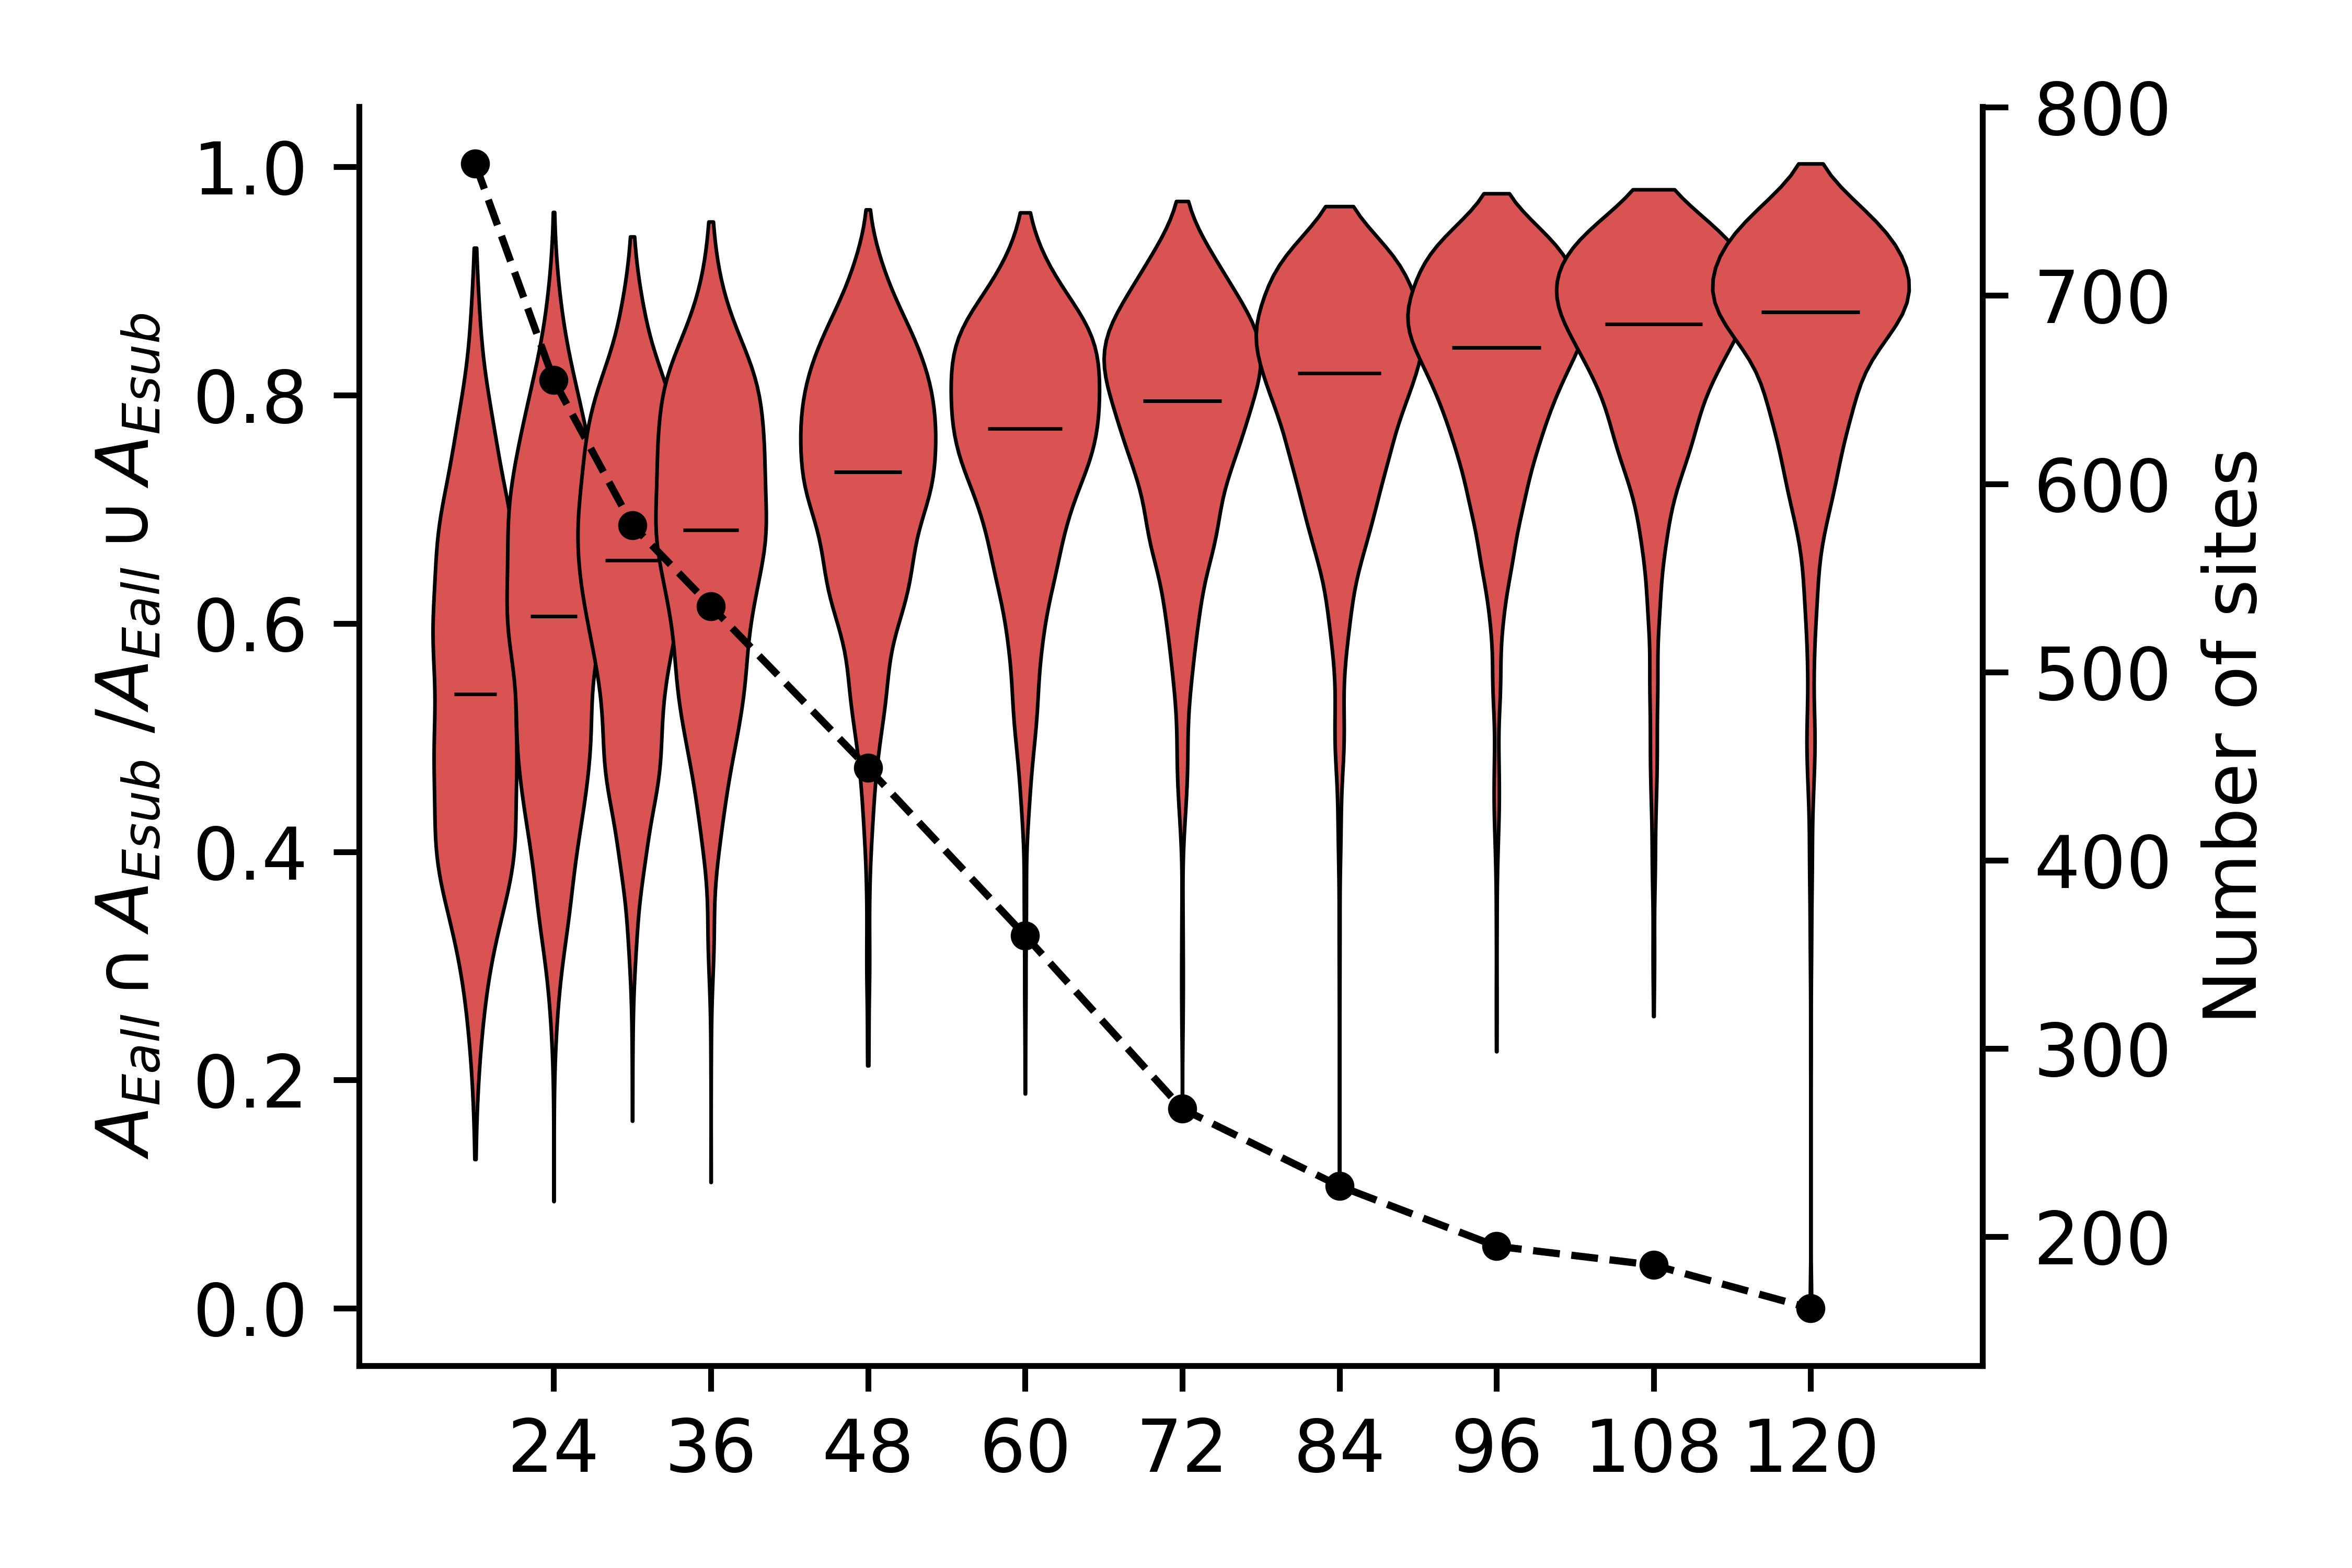
\includegraphics[width = 4.5in]{Figs/Fig1.png}
\caption{Violin plot comparison of the standardized overlap area for ellipses from subtimeseries, relative to the long term ellipse estimate. The numbers are scaled to the union of the subtimeseries and full timeseries ellipse areas, since the subtimeseries ellipse is usually larger than the full timeseries ellipse. Each violin shows the distribution of standardized ellipse overlap area results based on 1620 ellipse estimates. Longer violins indicate a wider range of overlap values for a given subtimeseries length, whereas wide parts of violins indicate a large number of subtimeseries comparisons shared that overlap value. The central dash indicates the median ellipse overlap. The number of sites available with records equal to or exceeding the thresholds is shown as the black line corresponding to the the right axis. }
\label{fig:ellipse}
\end{figure}

\begin{figure}
  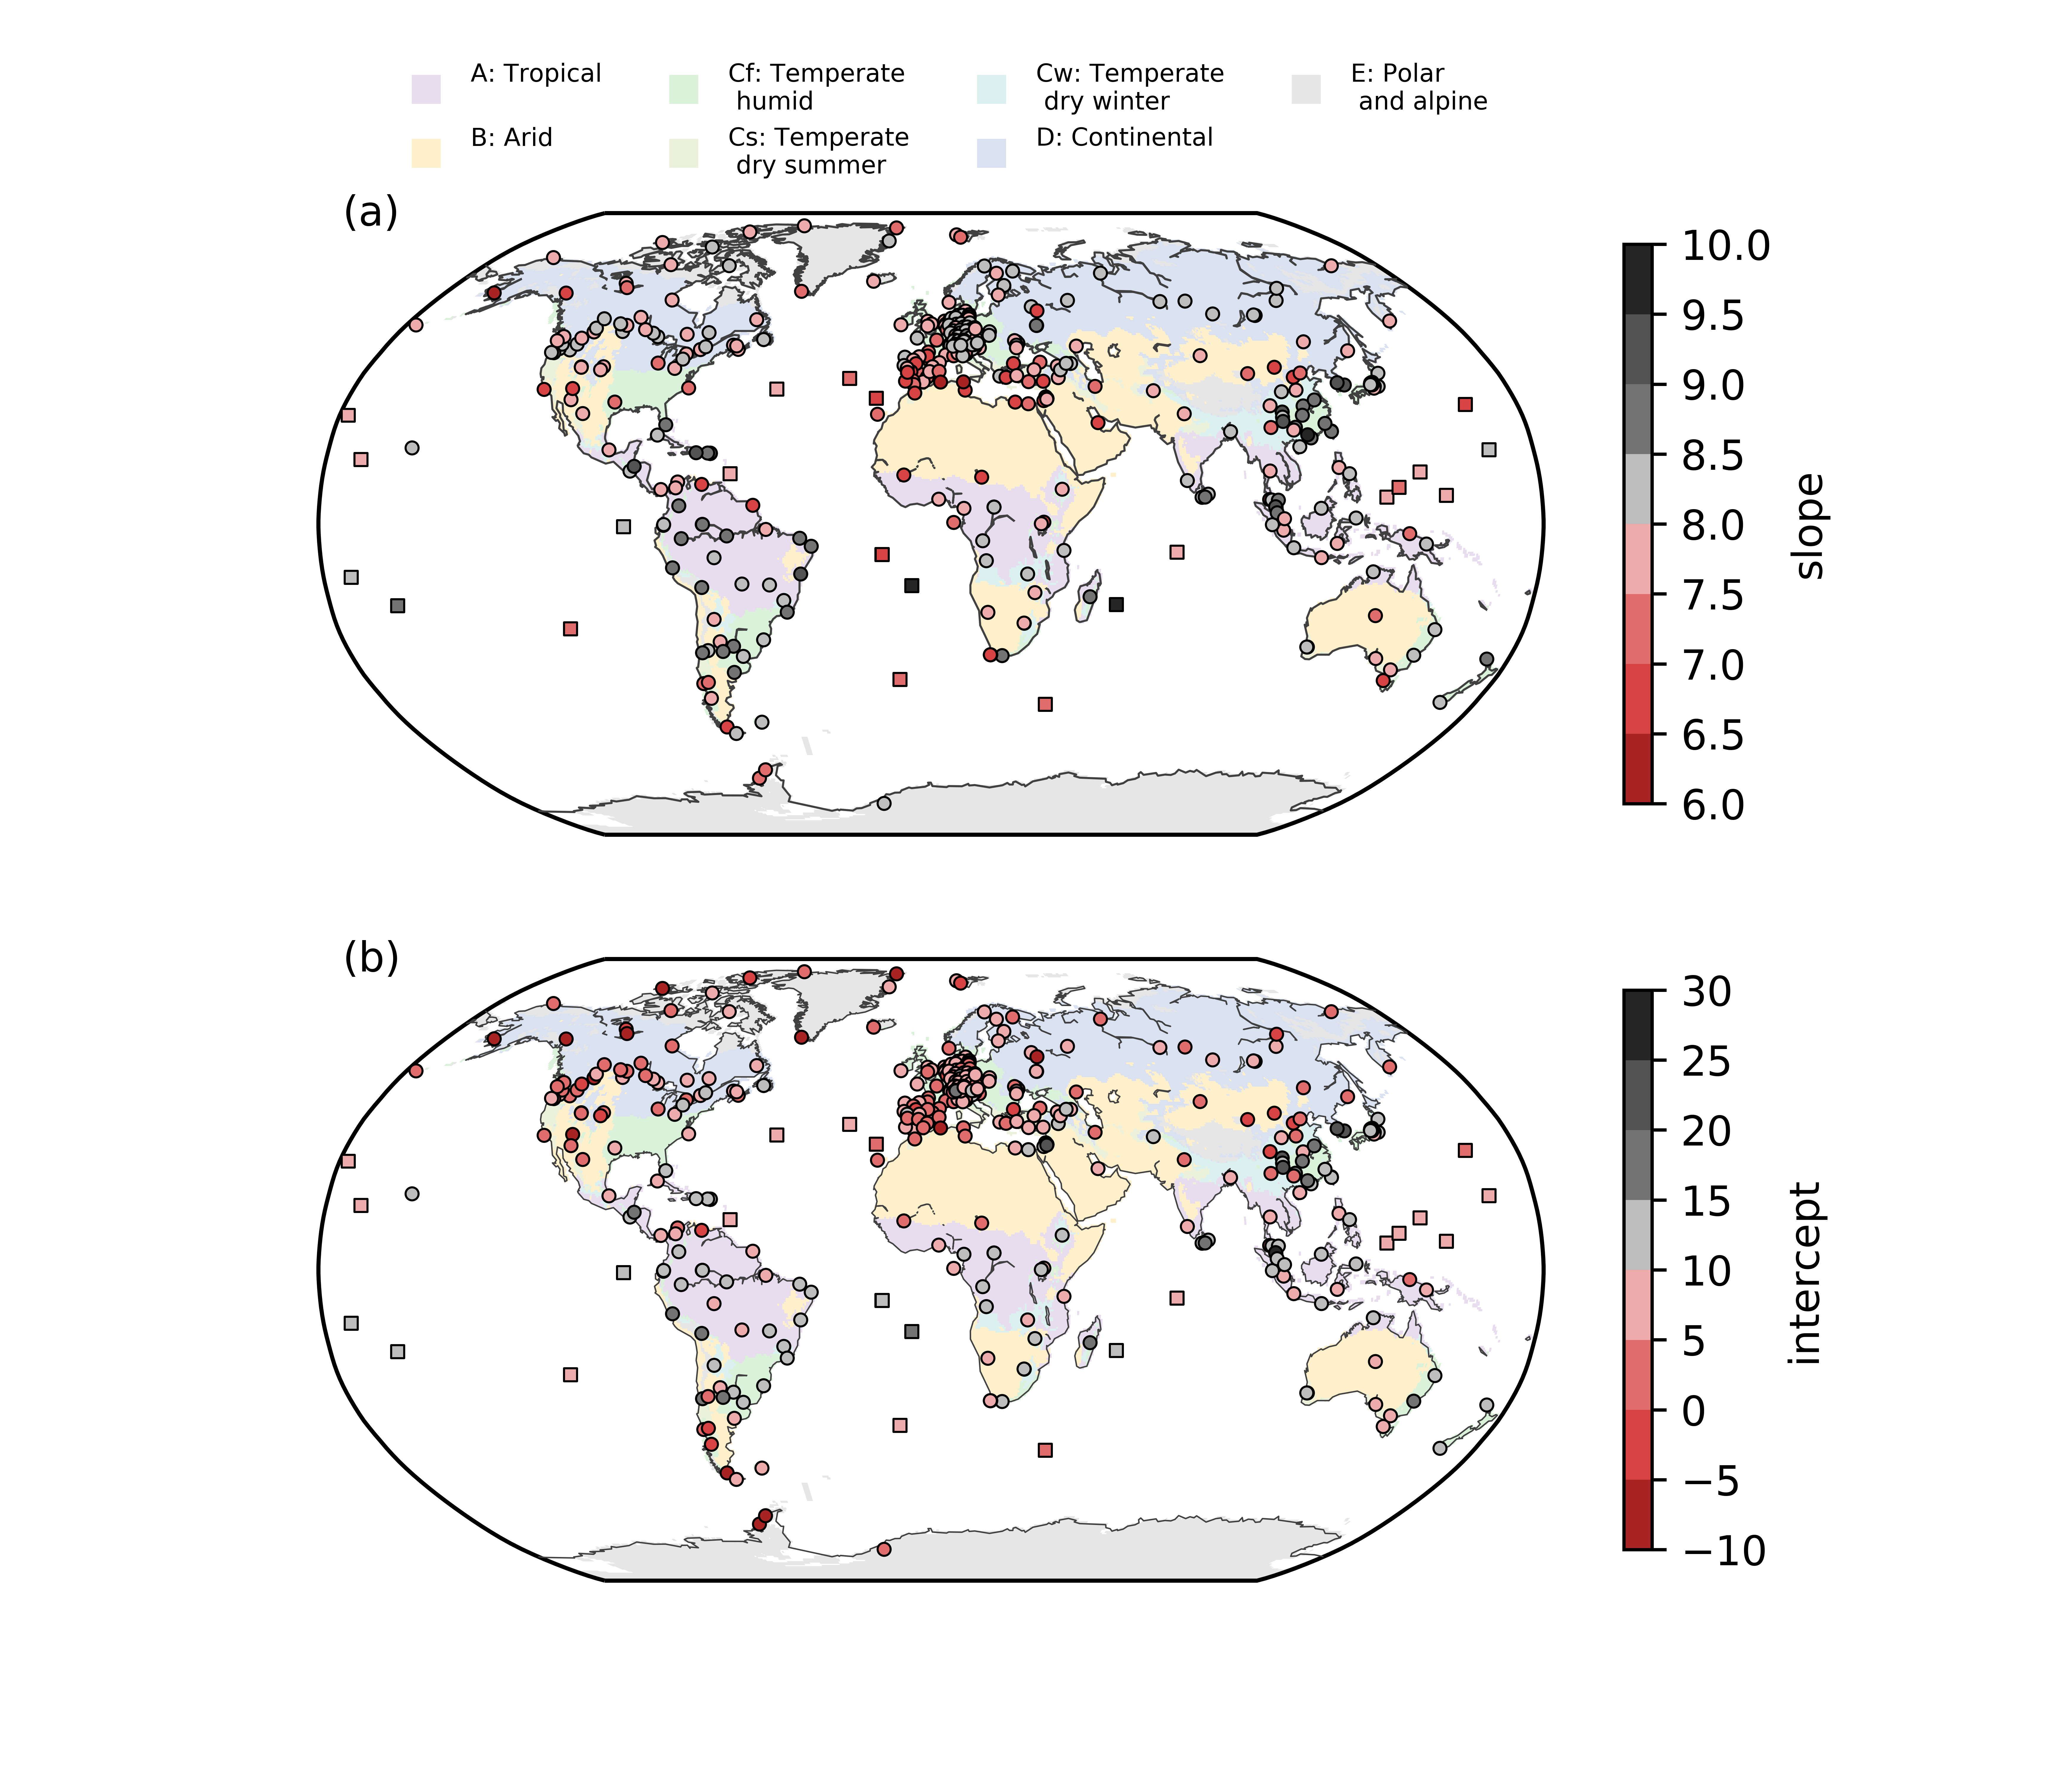
\includegraphics[width=7in]{Figs/Fig2.png}
  \caption{(a) Map of the global distribution of local meteoric water line slopes (b) and intercepts. The dataset is displayed over a simplified K{\"o}ppen climate classification map (colors are pastel hues of colors in subsequent figures). Square symbols occur where no K{\"o}ppen climate classification was assigned (denoted `N' in later figures), which occurred exclusively at island sites. The map includes sites that have at least 48 months of data, with data collected in every season where rainfall is expected. This figure shows the spatial distribution of sites and spatial structure of LMWL parameters, indicating that we have sufficient spatial representation for a global analysis, and robust representation of sites in different climate classes.}
  \label{fig:lmwlpoints}
\end{figure}

\begin{figure}
  \centering
  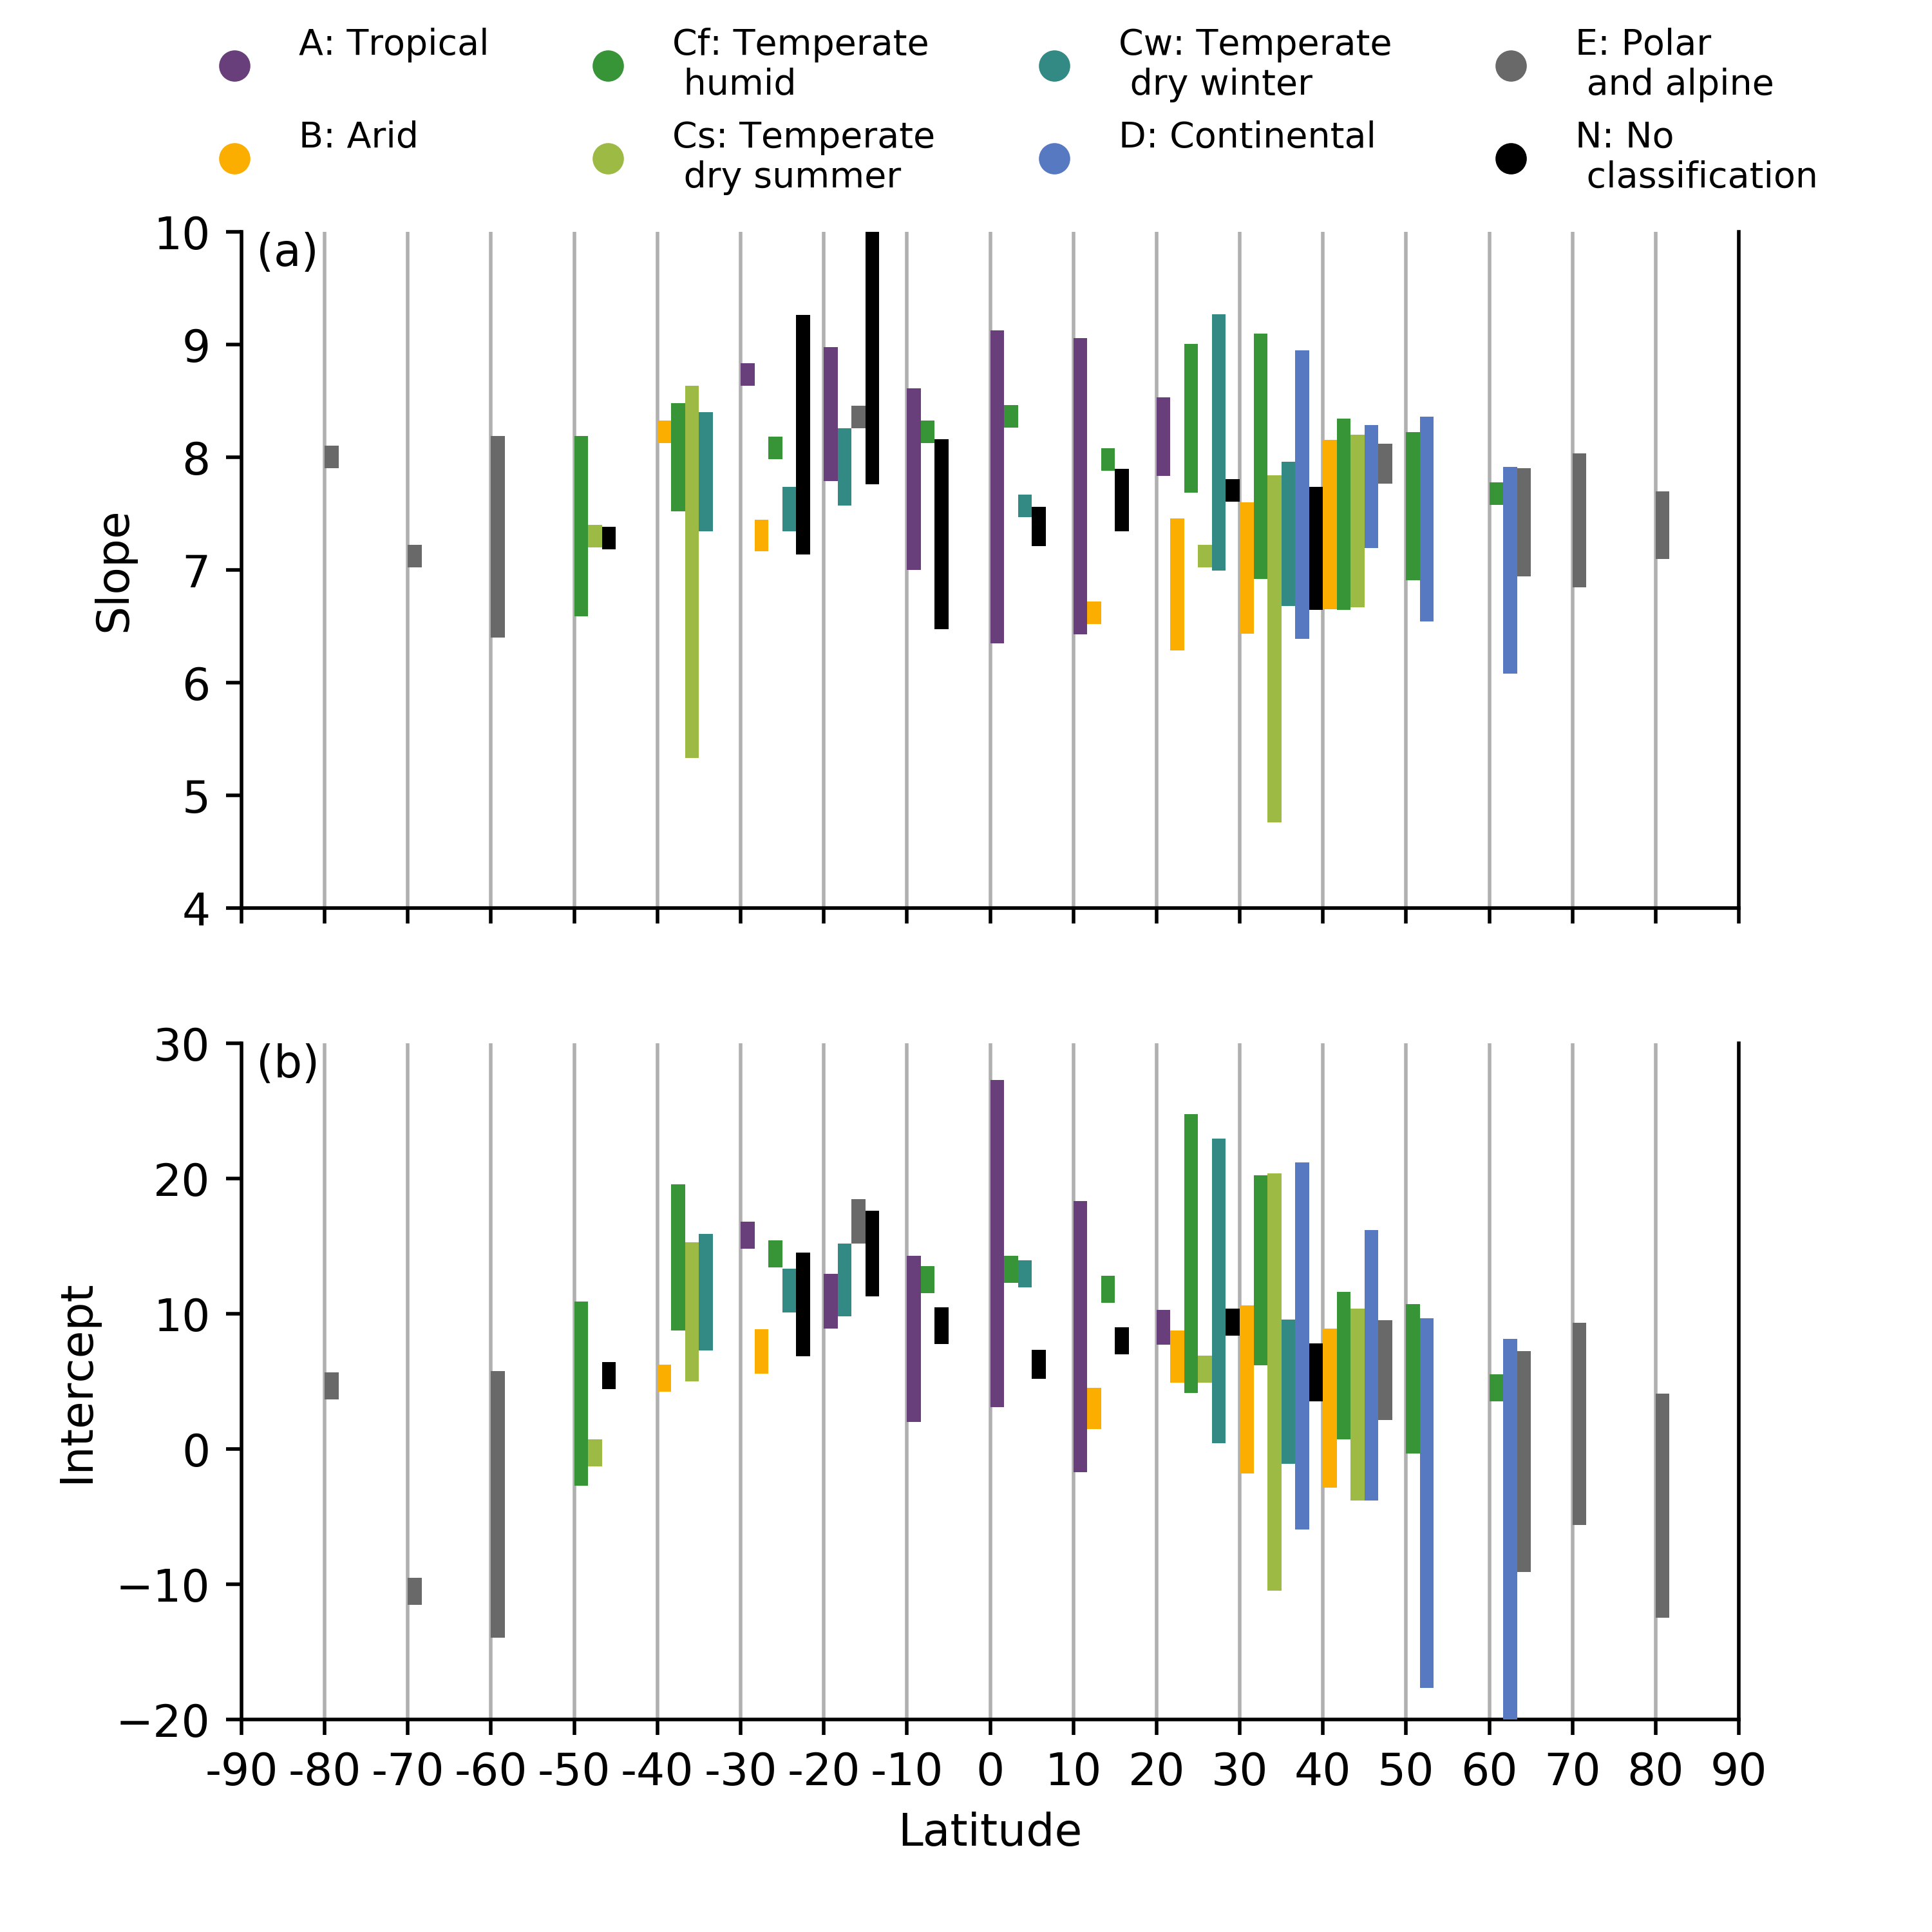
\includegraphics[width=6in]{Figs/Fig3.png}
  \caption{Distributions of local meteoric water line (a) slopes and (b) intercepts binned by latitude (bin edges shown with gray vertical lines) and grouped by K{\"o}ppen climate class. Hot or warm humid regions in the tropics and mid-latitudes (Climate classes A, Cf, and Cw) show the highest slopes, whereas arid and seasonally hot and dry regions (climate classes B and Cs) indicate the lowest slopes. The lowest intercepts occur in snowy regions (Climate classes D and E).}
  \label{fig:zonalboxplot}
\end{figure}

\begin{figure}
  \centering
  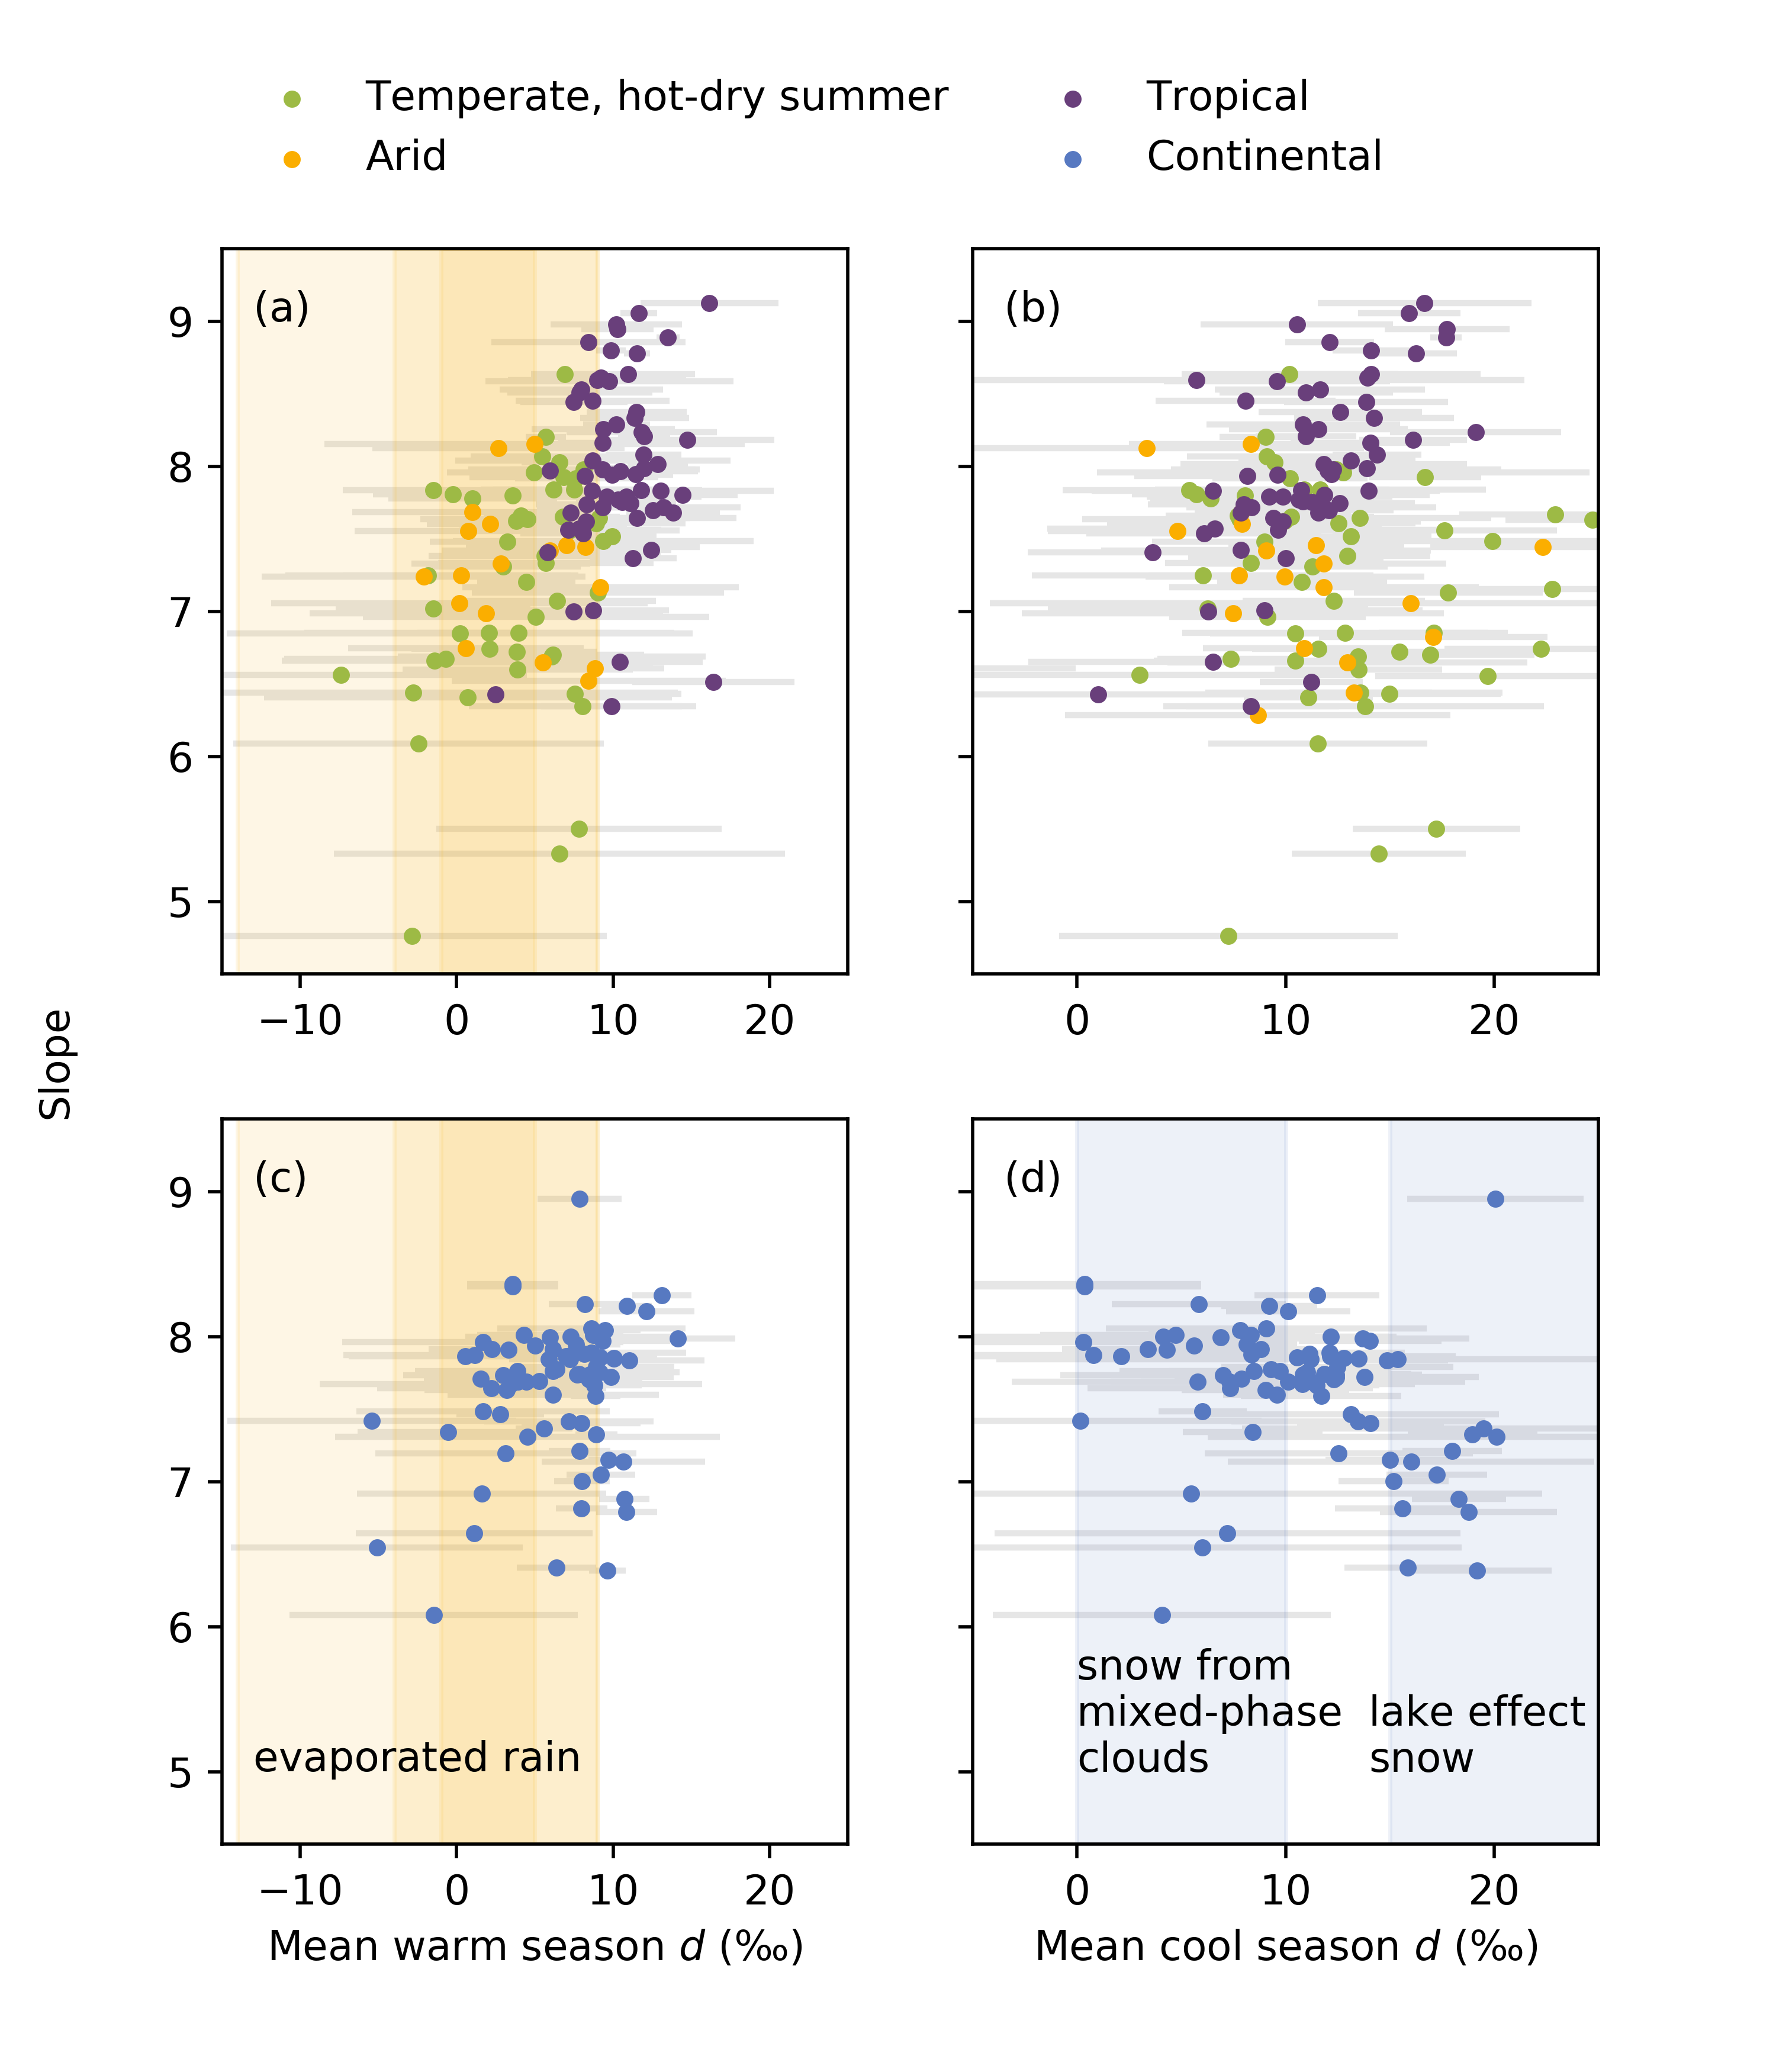
\includegraphics[width=6in]{Figs/Fig4.png}
  \caption{We link variation in slope to hydroclimatic processes via $d$. The processes producing different $d$ values vary with climate class and season. In panel (a) we compare the warm season $d$ for hot or warm humid regions in the tropics (Climate class A) with the warm season $d$ for arid and seasonally hot and dry regions (climate classes B and Cs). This data is shown on top of $d$ ranges (in yellow) from a set of studies~\citep{Chen2015, Wang2016, Graf2019} that indicated substantial sub-cloud evaporation contributed to the observed $d$. In panel (b) we show the same sites, but for the cool season. The comparison suggests that warm season differences in humidity drive differences in LMWL slope. (c) Warm and (d) cool season $d$ at continental, seasonally snowy regions (Climate class D) may influence slope. The blue shaded regions in panel (d) indicate the $d$ ranges predicted by~\citet{Ciais1994} for mixed phase cloud processes during Rayleigh distillation, and $d$ ranges resulting from lake effect snow~\citep{Corcoran2019}. Either high cool season $d$ or low warm season $d$ can result in lower slopes. }
  \label{fig:seasonaldex}
\end{figure}

\begin{figure}
  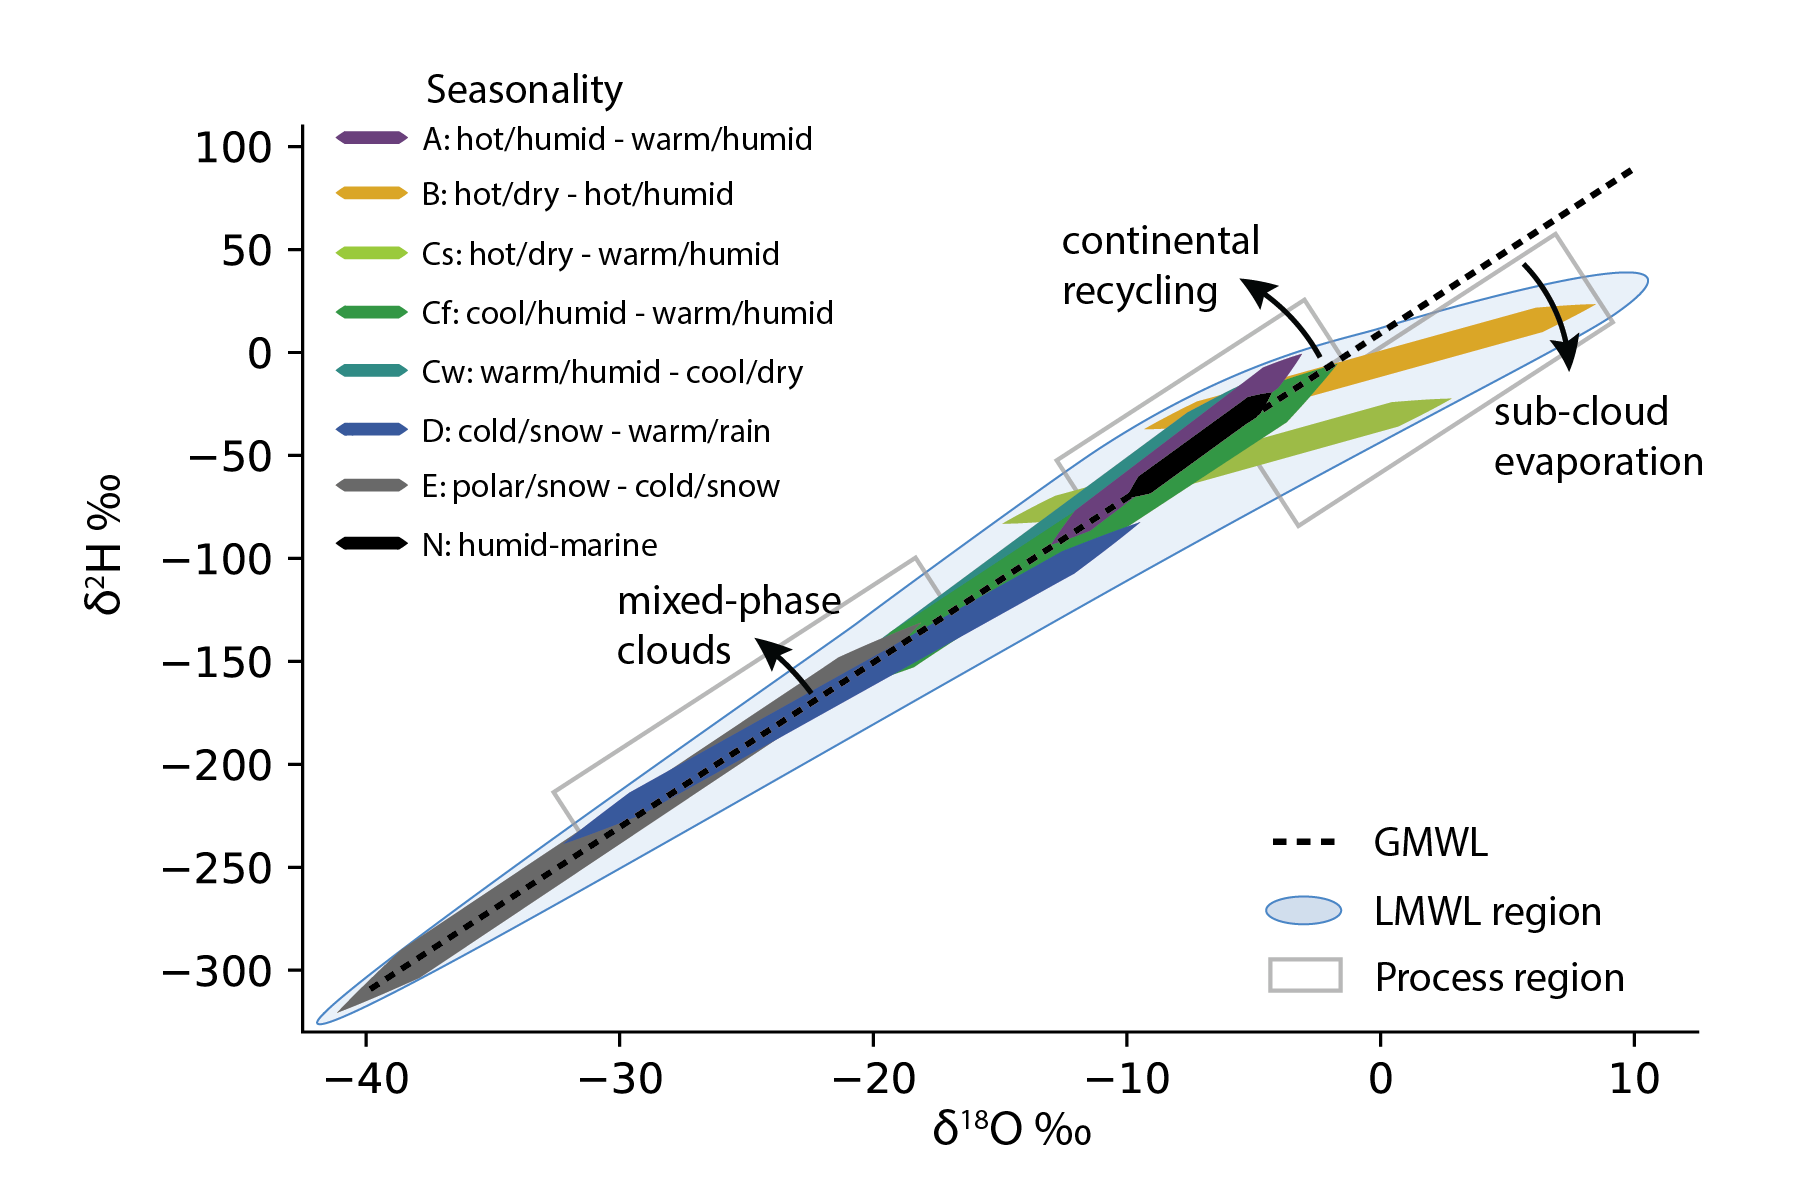
\includegraphics[width=6in]{Figs/Fig5.png}
  \caption{The region occupied by local meteoric water lines around the global meteoric water line. This schematic shows how local meteoric water lines from different K{\"o}ppen climate classes contribute to the shape of the local meteoric water line region. Each line represents a different idealized hydroclimatic scenario, with seasonal hydroclimatic extrema described in the key. In this figure, the code `N' represents the marine environment expected for island sites, since island sites comprise all unclassified sites. The regions of the plot most affected by the processes discussed in the text are indicated with a box and arrow, which shows which direction the process pulls the LMWL relative to the GMWL. The processes shown in the figure and discussed in the text may also occur in other regions, but exhibit a muted effect. }
  \label{fig:LMWLschematic}
\end{figure}


\begin{figure}
  \centering
  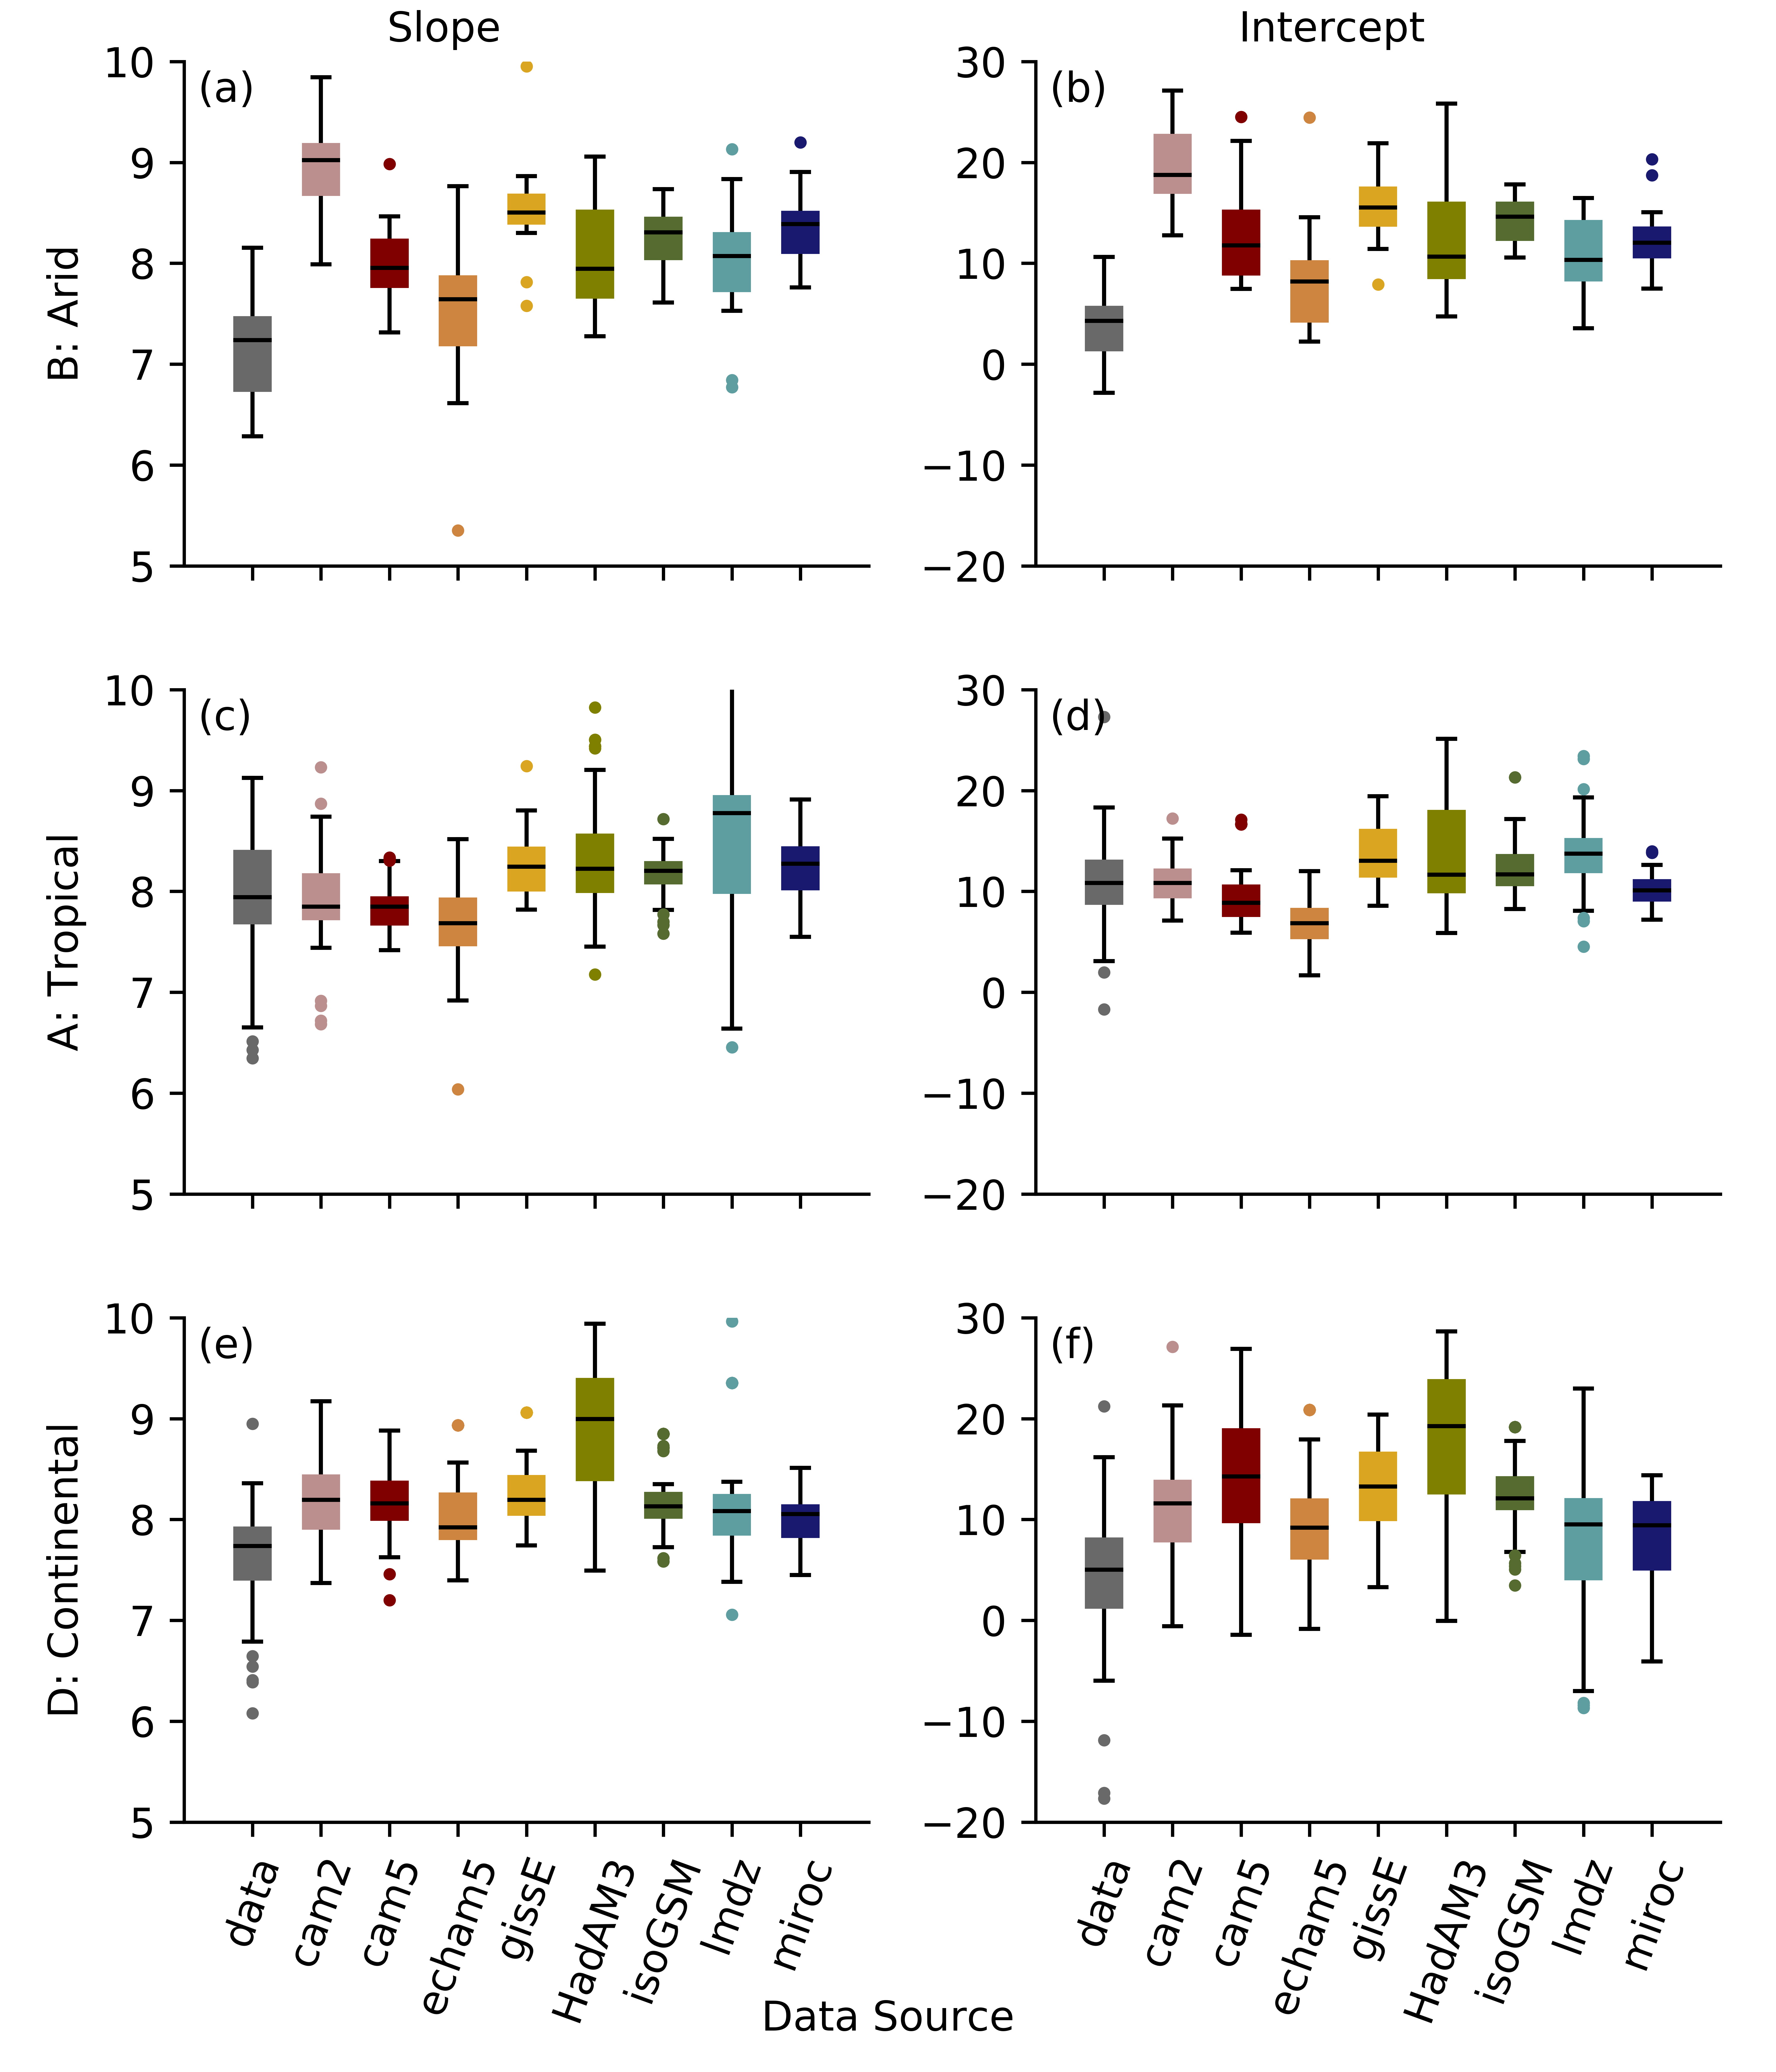
\includegraphics[width = 6in]{Figs/Fig6.png}
  \caption{Comparison of model data slope (a, c, e) and intercept (b, d, f) distributions with those from observational data, organized by K{\"o}ppen climate classification. In general, models tend to overestimate the slope and intercept in arid regions (panels (a) and (b), K{\"o}ppen class B)  relative to data. Slope and intercept estimates from model data in tropical regions (panels (c) and (d), K{\"o}ppen class A) match the observational data median well, but exhibit muted variability. Models tend to overestimate the slope and intercept of continental (panels (e) and (f), K{\"o}ppen class D) relative to data.}
  \label{fig:ModDataSubsets}
\end{figure}

\FloatBarrier
%tables:
\begin{sidewaystable}

\caption{Summary of isotope enabled climate models}
\centering
\begin{tabular}{ l || c  l  l }
\label{tab:modrefs}
Model Name & Native Resolution & Model Reference & Isotopic Reference \\
\hline
\hline
CAM2 & T42 ($\sim$2.8 x 2.8\textdegree) & \citet{Collins2002} & \citet{Lee2007} \\
CAM5 & 0.9 x 1.25\textdegree & \citet{Neale2010} & \citet{Nusbaumer2017}, \\
 & & & \citet{Wong2017}) \\
ECHAM5 & T106 ($\sim$1.1 x 1.1\textdegree) & \citet{Roeckner2003} & \citet{Steiger2017}\\
& & & \citet{Werner2011} \\
GISS ModelE & 2 x 2.5\textdegree & \citet{Schmidt2006} & \citet{Schmidt2007} \\
HadAM3 & 2.5 x 3.75\textdegree & \citet{Pope2000} & \citet{Tindall2009} \\
isoGSM & 2.5 x 2.5\textdegree & \citet{Kanamitsu2002} & \citet{Yoshimura2008} \\
LMDZ4 &	2.5 x 3.75\textdegree & \citet{Hourdin2006} & \citet{Risi2010} \\
MIROC &	T42 ($\sim$2.8 x 2.8\textdegree) & \citet{k-1_modeldevelopers} & \citet{Kurita2011} \\

% \multicolumn{2}{l}{$^{a}$Footnote text here.}
\end{tabular}
\end{sidewaystable}
\FloatBarrier
%%%%%%%%%%%%%%%%%%%%%%%%%%%%%%%%%%%%%%%%%%%%%%%%%%%%%%%%%%%%%%%%
%
%  ACKNOWLEDGMENTS
%
% The acknowledgments must list:
%
% >>>>	A statement that indicates to the reader where the data
% 	supporting the conclusions can be obtained (for example, in the
% 	references, tables, supporting information, and other databases).
%
% 	All funding sources related to this work from all authors
%
% 	Any real or perceived financial conflicts of interests for any
%	author
%
% 	Other affiliations for any author that may be perceived as
% 	having a conflict of interest with respect to the results of this
% 	paper.
%
%
% It is also the appropriate place to thank colleagues and other contributors.
% AGU does not normally allow dedications.
\acknowledgments
Data used in this project came from the Water Isotopes Database (waterisotopes.org). Original data may be accessed by querying Project\_ID's 00004, 00016, 00020, 00025, 00027, 00037, 00038, 00042, 00053, 00055, 00078, 00084, 00109, 00128, 00133, 00129, 00138, 00139, 00159, 00161, 00167 and 00169, and data may be downloaded where data owners have allowed their datasets to be publicly available and redistributable. We have also included a subset of the publicly available, processed data in the supplemental information. The authors thank all data contributors, as well as those who organized datasets for upload. All scripts and publicly available data can be accessed in the supplemental information or from https://github.com/putmanannie/LocalMeteoricWaterLines.
 
Support for this work was provided by US National Science Foundation grants EF-1241286, DBI-1565128. A.P. was supported by the University of Utah Graduate Research Fellowship program, and Z.C. was supported by the China Scholarship Council.

The authors declare no conflicts of interest.
 
\bibliography{LMWL.bib} 
\end{document}

